\documentclass[11pt,a4paper]{article}

\usepackage[T1]{fontenc}
\usepackage[utf8]{inputenc}
\usepackage{lmodern}
\usepackage[margin=2.4cm]{geometry}
\usepackage{amsmath,amssymb,amsthm,mathtools}
\usepackage{booktabs}
\usepackage{tabularx}
\usepackage{longtable}
\usepackage{array}
\newcolumntype{L}{>{\raggedright\arraybackslash}X}
\usepackage{enumitem}
\usepackage{xcolor}
\usepackage{tikz}
\usetikzlibrary{arrows.meta,positioning,calc,fit,backgrounds}
\usepackage[colorlinks=true,linkcolor=blue!45!black,citecolor=blue!45!black,urlcolor=blue!45!black]{hyperref}
\usepackage{microtype}
\usepackage{caption}
\usepackage{fancyhdr}
\usepackage{titlesec}

\definecolor{accent}{RGB}{20,52,96}
\definecolor{soft}{RGB}{238,242,247}

\titleformat{\section}{\normalfont\Large\bfseries\color{accent}}{\thesection}{0.8em}{}
\titleformat{\subsection}{\normalfont\large\bfseries\color{accent}}{\thesubsection}{0.7em}{}
\titleformat{\subsubsection}{\normalfont\normalsize\bfseries}{\thesubsubsection}{0.6em}{}

\pagestyle{fancy}
\fancyhf{}
\fancyhead[L]{\footnotesize Machine-checked dimension theory for fusion categories}
\fancyhead[R]{\footnotesize\thepage}
\renewcommand{\headrulewidth}{0.3pt}

\newtheorem{theorem}{Theorem}[section]
\newtheorem{proposition}[theorem]{Proposition}
\newtheorem{lemma}[theorem]{Lemma}
\newtheorem{corollary}[theorem]{Corollary}
\newtheorem{definition}[theorem]{Definition}
\newtheorem{conjecture}[theorem]{Conjecture}
\newtheorem{question}[theorem]{Question}
\theoremstyle{remark}
\newtheorem{remark}[theorem]{Remark}
\newtheorem{example}[theorem]{Example}

\newcommand{\code}[1]{\texttt{\detokenize{#1}}}
\newcommand{\C}{\mathcal{C}}
\newcommand{\D}{\mathcal{D}}
\newcommand{\Id}{\mathrm{Id}}
\newcommand{\FPdim}{\mathrm{FPdim}}
\newcommand{\Vect}{\mathrm{Vec}}
\newcommand{\one}{\mathbf{1}}
\newcommand{\dual}[1]{#1^{*}}
\newcommand{\dd}[1]{#1^{**}}
\newcommand{\field}{\Bbbk}
\newcommand{\R}{\mathbb{R}}
\newcommand{\Cx}{\mathbb{C}}
\newcommand{\Z}{\mathbb{Z}}
\newcommand{\N}{\mathbb{N}}
\newcommand{\Q}{\mathbb{Q}}

\setlength{\emergencystretch}{3em}

\setlist[itemize]{topsep=2pt,itemsep=1pt,parsep=0pt}
\setlist[enumerate]{topsep=2pt,itemsep=2pt,parsep=0pt}

\title{\vspace{-1.2cm}\textbf{Machine-Checked Dimension Theory\\ for Fusion Categories}\\[0.35cm]
\large A research proposal: pivotal and spherical structures, the double-dual twist,\\ and a verified proof of Etingof--Nikshych--Ostrik Proposition~8.23}
\author{Tzu-Chen Huang}
\date{November 2026 \quad\textbar\quad proposal v1.2 (second revision) \quad\textbar\quad repository state \texttt{d3d320e}}

\begin{document}

\maketitle

\begin{abstract}
\noindent
This proposal sets out a research programme whose central target is the first machine-checked
proof of Etingof--Nikshych--Ostrik Proposition~8.23: \emph{every pseudo-unitary fusion
category admits a unique spherical structure whose dimensions are the Frobenius--Perron
dimensions}. The theorem is the standard bridge from an analytic hypothesis (one scalar
equation on the global dimension) to the algebraic structure that all of dimension theory
presupposes, and it is used as a black box throughout the classification literature. No
formal proof of it exists, and the categorical infrastructure on which it rests is only now
arriving in Mathlib.

The programme builds on substantial preliminary work, reported in \S\ref{sec:prelim}: a
skeletal formalisation of multiplicity-free rigid fusion data with a proved inhabitant; a
corrected duality normalisation that inhabits Fibonacci and Ising over $\R$; a reduction of
the target to a single per-channel identity on the double-dual twist; a formalised proof of
ENO Proposition~8.21; and a reconstruction of ENO's route through the square root $a$ of the
quadruple-dual isomorphism, together with the identification of ENO's trace identity with
multiplicativity of the dimension. One of these results is negative and changes the shape of
the target: ENO~8.23 is \emph{false} without its pseudo-unitarity hypothesis (a kernel-checked
two-simple counterexample, the Yang--Lee category). A second witness shows that the dimension
function depends on the choice of pivotal structure although the fusion ring is unchanged.
The proposal turns these findings into a three-aim programme: a corrected and inhabitable
formal signature together with its bridge to Mathlib's emerging pivotal and spherical
category theory; a derivation of the double-dual twist from the duality data; and a
formalisation of ENO's analytic core, yielding Proposition~8.23 in the scope actually
formalised --- multiplicity-free data, with the analytic theorem stated over $\Cx$ (FP
dimensions embedded from $\R$, positivity defined once), and the quadruple-dual theorem
either taken as a hypothesis or proved by Bartlett's string-diagram argument.

The scope is narrower than the title of the source theorem and is fixed in \S\ref{sec:scope}:
multiplicity-free data; the algebraic layer over a field of characteristic zero with the
analytic theorem over $\Cx$; and the quadruple-dual isomorphism either
as a hypothesis or proved by Bartlett's string-diagram argument. The 24-month schedule is ordered
by risk --- corrected signature and exact target, reconstruction and trace correspondence, derived
twist, ENO's normalisation --- and the deliverables include an axiom-clean Lean~4 library, a
verified negative-result note, upstream Mathlib contributions, and a documented methodology for
auditing formal statements against their sources.

\end{abstract}

\vspace{0.2cm}

\begin{center}
\begin{minipage}{0.94\textwidth}
\colorbox{soft}{%
\begin{minipage}{0.92\textwidth}
\vspace{0.12cm}
\footnotesize
\textbf{At a glance.}\par\vspace{2pt}
\begin{tabularx}{\textwidth}{@{}lL@{}}
\textbf{Object} & Pivotal and spherical structures on fusion categories, and ENO Prop.~8.23.\\
\textbf{Method} & Skeletal finite data in Lean~4 (pinned to Mathlib \texttt{0df444a3}); exact arithmetic in
$\Z[\sqrt d]$; kernel-checked counterexamples; axiom audit; bridge to Mathlib's categorical layer.\\
\textbf{Already done} & $\sim$5{,}200 lines, 23 modules; a green 3{,}032-job build at \texttt{d3d320e}
(not yet a reproduced clean build); 73 audited declarations at
\texttt{[propext, Classical.choice, Quot.sound]}; no \texttt{sorry}.\\
\textbf{Still open} & A corrected signature and an exact target; the twist derivation (the
$\Omega$ formula in \texttt{PLAN.md} is retracted); the $\Cx$ scalar contract; the reconstruction and
trace correspondence; ENO's $\sigma/\tau$ normalisation; the quadruple-dual theorem.\\
\textbf{Horizon} & 24 months, 7 work packages, 12 numbered deliverables; a first delegation
batch (B1--B4, \S\ref{sec:batch}) gates all dependent theorem work.\\
\end{tabularx}
\vspace{0.15cm}
\end{minipage}}
\end{minipage}
\end{center}

\newpage

{\footnotesize\tableofcontents}

\newpage

\section{Introduction}

\subsection{Dimension theory sits between decidable combinatorics and open structure}

A fusion category over a field $\field$ is a $\field$-linear, semisimple, rigid monoidal category with
finitely many simple objects and $\mathrm{End}(\one) = \field$. Its Grothendieck ring $K_0(\C)$ is
finite, decidable data: a finite set $I$ of simples, integers $N_{ij}^k = \dim \mathrm{Hom}(X_k, X_i
\otimes X_j)$, a duality involution $i \mapsto i^*$. Almost everything one wants to compute about
$\C$ --- dimensions, the global dimension, Frobenius--Schur indicators, the $T$-matrix of a
modular category, the state sum of a three-manifold --- depends on more than this ring, but less
than the full category.

The intermediate datum is a \emph{pivotal structure}: a monoidal isomorphism
$\gamma \colon \Id \to (-)^{**}$. It yields a dimension $\dim_\gamma(X) = \mathrm{tr}(\gamma_X)$
for every object, and a \emph{spherical} structure --- one with $\dim_\gamma(X) =
\dim_\gamma(\dual{X})$ --- is what makes the trace cyclic and therefore produces invariants of
oriented manifolds rather than of framed ones.

Two facts locate the research problem precisely.

\begin{enumerate}[label=(\alph*)]
\item \emph{The dimension function is not a function of the fusion ring.} This is not a
philosophical remark: the present project contains a kernel-checked witness
(\S\ref{sec:prelim}, \code{VecZ2Twisted}). The category $\Vect^\omega_{\Z/2}$ with non-trivial
cocycle carries two pivotal structures whose dimensions on the non-trivial simple are $+1$ and
$-1$ respectively. Any formalisation that treats ``the dimension'' as determined by the fusion
rules is therefore wrong, and the first version of this project's pivotal axiom was wrong in
exactly that way.
\item \emph{Whether a pivotal structure exists is open in general.} Etingof--Nikshych--Ostrik
conjectured that every fusion category is pivotal (ENO, Conjecture~2.8); the spherical
strengthening is stronger still. What is known is a sufficient condition of a different
character: pseudo-unitarity.
\end{enumerate}

\subsection{The theorem that bridges the two}

ENO Proposition~8.23 states that a pseudo-unitary fusion category --- one whose categorical
global dimension equals its Frobenius--Perron global dimension --- admits a \emph{unique}
pivotal structure, which is spherical, and with respect to which the categorical dimensions of
all simple objects are positive and equal to their Frobenius--Perron dimensions.

The proposition is used as a black box across the classification programme: in Ostrik's
analysis of pivotal fusion categories of rank~3 and the resulting inequality, in the
Haagerup--Izumi existence problem, in the passage from unitary anyon data to modular data, and
in every place where one writes down a spherical category from a fusion ring plus positivity.
It is, in a precise sense, the lemma that makes the rest of the subject work.

\subsection{Why formalise, and why this is not transcription}

A referee reading a two-page proof in a 2005 Annals paper cannot check, line by line, that the
gauge chosen for the associator is the one in which the evaluation and coevaluation have the
normalisation the argument assumes. A proof assistant can. The empirical case for this
proposal is that when the present project first wrote down the statement, four defects
surfaced, every one of them invisible to a reader checking that the formulas \emph{looked}
right:

\begin{enumerate}[label=\textbf{D\arabic*.},leftmargin=2.2em]
\item \textbf{The signature had no inhabitants.} The two unit axioms of the skeletal fusion
datum were mutually inconsistent for $n \ge 2$: evaluated at $(0,b,0,d,b,0)$ they forced
$1 = 0$. Every theorem quantified over the structure was therefore vacuous, including a
``proof'' of the target theorem.
\item \textbf{The pentagon was not the pentagon.} The axiom called \code{pentagon} had eight
free labels where the $F$-matrix pentagon requires ten, and it fails on
$\Vect^{\omega}_{\Z/2}$ for \emph{every} cocycle $\omega$, the trivial one included. A green
build certified a false axiom.
\item \textbf{The pivotal axiom fixed the twist to one.} \code{p_fusion} assumed
$J \equiv 1$, where $J$ is the monoidal structure of $(-)^{**}$. With that assumption every
fusion-rule table is pivotal via $p \equiv 1$, and the target theorem became provable with no
hypothesis at all --- the formal statement had drifted so far from the source that it asserted
something false.
\item \textbf{The second snake used the wrong inverse.} It wrote the right snake with a
reciprocal of an associator \emph{entry} where the $(0,0)$-entry of the \emph{matrix inverse} of
the associator block is required. The two agree for pointed categories and differ for
Fibonacci, so the axiom excluded the two principal examples.
\end{enumerate}

Each defect was found by making the statement inhabitable and checking it against the examples,
not by re-reading it. This is the methodological thesis of the proposal: in this subject the
value of formalisation lies less in the final certificate than in the audit that produces it,
and the audit is transferable.

\subsection{What has already been established}\label{sec:whatdone}

The preliminary results of \S\ref{sec:prelim} are not a plan; they are a library. In summary:

\begin{itemize}
\item a skeletal signature for multiplicity-free rigid fusion data, with a proved inhabitant
($\Vect_{\Z/2}$) and the pentagon checked on all $512$ label tuples;
\item a corrected duality normalisation, with the inverse associator carried as data, that
inhabits Fibonacci and Ising over $\R$ --- every field proved, including both snakes --- and
yields the spherical pivotal structure with $\dim = \FPdim$ for both;
\item a proof that a pivotal dimension is always a coboundary of the normalised double-dual
twist, and that ENO~8.23 is \emph{equivalent} to one per-channel identity on that twist;
\item a formalised ENO Proposition~8.21: the spectral bound $|d_i| \le \FPdim_i$ for any
dimension function satisfying the eigenvector equation, together with the equality case;
\item a kernel-checked refutation of the target as stated without hypotheses (Yang--Lee), and a
second witness that the dimension function is not determined by the fusion ring;
\item a reconstruction of ENO's own proof route --- the square root $a$ of the quadruple-dual
isomorphism, its monoidality defect $b$, and the trace identity --- together with a proof that
ENO's trace identity \emph{is} the multiplicativity identity that the twist reduction isolates.
\end{itemize}

The library builds (3{,}032 jobs, warnings only), contains no \texttt{sorry}, and its axiom
audit over 73 declarations reports \texttt{[propext, Classical.choice, Quot.sound]} throughout.

\subsection{What is not yet established}

The gap is now sharp, and it is not the algebra. It is ENO's analytic argument: the passage from
the pseudo-unitarity equation (one scalar identity, Definition~\ref{def:pseudo}) to a dimension
function that is positive and multiplicative. Proposition~8.21 turns the \emph{sum} equality
$\sum_i |d_i|^2 = \sum_i \FPdim_i^2$ into a termwise equality $|d_i| = \FPdim_i$; a tensor
automorphism of the identity, $\sigma = d^2/|d|^2$, then makes the dimensions real, and a
\emph{natural} automorphism $\tau = d/|d|$ --- not monoidal in general --- makes them positive.
No Hermitian structure enters the hypothesis or the proof: positivity is part of what the
argument \emph{produces}, and an earlier draft of this section described the gap as a passage
from a Hermitian structure; that description is removed here and in the plan.
Alongside it, and logically prior to it, sit two defects of the signature rather than of the
mathematics: the twist $J$ is carried as data constrained by four laws, not derived from
$(\mathrm{ev}, \mathrm{coev}, F)$, and the scalars are real where the source theorem is over
$\C$. Until $J$ is derived, the statement ``$p$ is pivotal'' mentions an object the
mathematics does not fix.

The scope is narrower than the source theorem and is fixed here once (\S\ref{sec:scope}):
multiplicity-free data; the algebraic layer over a field of characteristic zero with the
analytic theorem over $\Cx$ (S2 of \S\ref{sec:scope}); and the quadruple-dual isomorphism $g$
of ENO Theorem~2.6 either taken as a hypothesis or proved by the string-diagram argument of
Bartlett \S3.6. These are deliverables to be discharged, not silent assumptions.

\subsection{Research questions}

\begin{description}[leftmargin=1.6em,style=nextline]
\item[Q1 (Signature).] What is the weakest finite-data signature that is (i) inhabited by the
standard examples, (ii) strong enough to express pivotality and sphericity faithfully, and
(iii) provably equivalent to the abstract categorical notion?
\item[Q2 (Twist).] Is the double-dual twist $J$ determined by $(F, \mathrm{ev}, \mathrm{coev})$?
If so, what is its closed form, and does it satisfy the multiplicativity identity (M)?
\item[Q3 (Analytic core).] Can ENO's proof of Proposition~8.23 be carried out inside the
skeleton, taking as input only the pseudo-unitarity equation $\dim \C = \FPdim \C$?
\item[Q4 (Frontier).] What is the largest statement provable \emph{without} pseudo-unitarity ---
that is, what exactly is the content of ENO Conjecture~2.8 in a pivotal-free formalism, and
which of its consequences survive as theorems about torsion in the universal grading group?
\item[Q5 (Method).] Which failure modes of formalising monoidal category theory are
systematic, and can they be detected mechanically rather than by luck?
\end{description}

\subsection{Structure of the proposal}

\S\ref{sec:background} fixes notation and states the target precisely. \S\ref{sec:prior}
surveys prior work, mathematical and formal. \S\ref{sec:prelim} reports the preliminary
results in enough detail to be checked. \S\ref{sec:programme} sets out the seven work packages
and their milestones. \S\ref{sec:techniques} describes the techniques, including the ones that
failed. \S\ref{sec:risk}--\S\ref{sec:deliverables} give risks, timeline and deliverables.
\S\ref{sec:significance} argues for significance. Three appendices record the module
inventory, the audit protocol, and the Lean statements of the main targets.

\section{Background}\label{sec:background}

\subsection{Fusion categories and fusion rings}

\begin{definition}
A \emph{fusion category} over a field $\field$ is a $\field$-linear abelian, semisimple, rigid monoidal
category $\C$ with finitely many isomorphism classes of simple objects, such that
$\mathrm{End}_\C(\one) \simeq \field$ and the tensor product is bilinear and exact in each variable.
We write $I$ for the set of isomorphism classes of simples, $X_i$ for a representative, $0 \in I$
for the class of $\one$, and $i \mapsto i^*$ for the duality involution determined by
$\mathrm{Hom}(X_i \otimes X_j, \one) \neq 0 \iff j = i^*$.
\end{definition}

The Grothendieck ring $K_0(\C)$ has $\Z$-basis $(X_i)$ and structure constants
\[
X_i X_j = \sum_{k \in I} N_{ij}^{k} X_k, \qquad N_{ij}^k = \dim_\field \mathrm{Hom}(X_k, X_i \otimes X_j) \in \N .
\]
In this proposal a \emph{fusion ring} is the resulting abstract datum
$R = (N, (-)^*, 0)$: the multiplicities, the duality involution, and the unit. The axioms used
are those of a based ring: $N_{ij}^0 = \delta_{j,i^*}$; associativity
$\sum_k N_{ij}^k N_{kl}^m = \sum_k N_{jl}^k N_{ik}^m$; and compatibility of the involution with
the product. Commutativity is \emph{not} assumed.

\begin{definition}
A fusion ring is \emph{multiplicity-free} if $N_{ij}^k \in \{0,1\}$ for all $i,j,k$. It is
\emph{pointed} if every simple object is invertible, i.e.\ $N_{ij}^k \in \{0,1\}$ and
$\sum_k N_{ij}^k = 1$ for all $i,j$.
\end{definition}

Multiplicity-freeness is not a convenience in this project: with $N > 1$ the associator is a
matrix between multi-dimensional Hom spaces, and a single scalar $F^{abc}_d(e,f)$ cannot hold
it. The restriction is discussed in \S\ref{sec:tech-mult}.

\subsection{The Frobenius--Perron dimension}

\begin{theorem}[Frobenius--Perron, for fusion rings]\label{thm:pf}
Let $R$ be a fusion ring with $n$ classes. There is a unique function $f \colon I \to \R_{>0}$
with $f_0 = 1$ and
\begin{equation}\label{eq:fpchar}
f_i f_j = \sum_{k} N_{ij}^{k} f_k \qquad \text{for all } i,j \in I .
\end{equation}
Moreover $f_{i^*} = f_i$, each $f_i$ is an algebraic integer, and if the fusion graph is
connected then $f$ is the Perron--Frobenius eigenvector of every fusion matrix.
\end{theorem}

The number $f_i$ is the \emph{Frobenius--Perron dimension} $\FPdim(X_i)$, and
$\FPdim(\C) = \sum_i f_i^2$ is the Frobenius--Perron global dimension. Note that
\eqref{eq:fpchar} is the \emph{character} form: $f$ is a ring homomorphism $K_0(\C) \to \R$.

In the present library Theorem~\ref{thm:pf} is not proved: the existence and uniqueness of $f$
is packaged as a structure \code{FPData}, supplied by hand for each example. Discharging it from
Mathlib's Perron--Frobenius development is a deliverable (\S\ref{sec:programme}, WP0), not a
research risk: the relevant material exists upstream as a chain of pull requests
(\S\ref{sec:prior}).

\subsection{Duality, pivotal structures, and the double-dual twist}\label{sec:pivotaldef}

Rigidity supplies, for each object $X$, an evaluation $\mathrm{ev}_X \colon \dual{X} \otimes X
\to \one$ and a coevaluation $\mathrm{coev}_X \colon \one \to X \otimes \dual{X}$ satisfying the
two snake equations. In a skeleton, both are scalars, and the composite
\[
\kappa_i \;=\; \mathrm{ev}_i \cdot \mathrm{coev}_i \;\in\; \field^\times
\]
is the loop scalar of $X_i$. It is \emph{not} the dimension: the dimension depends on a choice
of identification of $X$ with its double dual.

\begin{definition}
A \emph{pivotal structure} on $\C$ is a monoidal natural isomorphism
$\gamma \colon \Id_\C \to (-)^{**}$. Its \emph{dimension} is
$\dim_\gamma(X) = \mathrm{tr}(\gamma_X \colon X \to X^{**})$, computed as the composite of
$\gamma_X$ with the evaluation of the right dual. The structure is \emph{spherical} if
$\dim_\gamma(X) = \dim_\gamma(\dual{X})$ for every $X$.
\end{definition}

Two remarks are essential and both cost the project a rewrite.

\begin{remark}[The twist]\label{rem:twist}
The functor $(-)^{**}$ is monoidal, and its monoidal structure is \emph{not} the identity. Write
$J_{ij}^{k}$ for the scalar of $X_i^{**} \otimes X_j^{**} \to (X_i \otimes X_j)^{**}$ on the
channel $k$. Then a pivotal structure on a skeleton is exactly a family
$(p_i)_{i \in I} \subset \field^\times$ with
\begin{equation}\label{eq:pivotal}
p_0 = 1, \qquad p_k = J_{ij}^{k}\, p_i\, p_j \quad \text{whenever } N_{ij}^k > 0,
\end{equation}
and the resulting dimension is
\begin{equation}\label{eq:dim}
\dim_i \;=\; p_i \, \kappa_i .
\end{equation}
Sphericity becomes
\begin{equation}\label{eq:sph}
\dim_{i^*} = \dim_i \ \ \forall i
\qquad\Longleftrightarrow\qquad
\kappa_{i^*} = p_i^{2}\, \kappa_i \ \ \forall i .
\end{equation}
\end{remark}

\begin{remark}[The trap]\label{rem:trap}
Two statements are easily conflated, and the project conflated them once. (i) \emph{Objectwise},
every simple object $V$ of a fusion category is isomorphic to its double dual $V^{**}$ (ENO
Proposition~2.1): the right dual $V^*$ is the unique simple $X$ with $V \otimes X \ni \one$, the
left dual ${}^*V$ is characterised the same way, and semisimplicity gives ${}^*V = V^*$, whence
$V \simeq V^{**}$. Consequently a skeleton may always be chosen with $i^{**} = i$ on the nose,
and the signature does not restrict generality by assuming it. (ii) \emph{Monoidally}, the
functor $(-)^{**}$ need not be isomorphic to the identity, and a monoidal such isomorphism is
\emph{precisely} a pivotal structure. Statement (i) fixes the objects and says nothing about
the monoidal structure; that structure is the twist $J$, and it is why $J$ is data.
An earlier version of this project built (ii) into the signature as $J \equiv 1$, which made
every fusion-rule table pivotal and the target theorem true without hypotheses; the claim that
a skeleton can always be chosen with $(-)^{**} = \mathrm{id}$ \emph{monoidally} is false, and it
is retracted in \texttt{PLAN.md}.
\end{remark}

\subsection{Pseudo-unitarity and the target}

\begin{definition}[Squared norms; ENO \S2.1, \S8.4; EGNO Definition~9.4.4]\label{def:pseudo}
For a simple $V$ and any isomorphism $a \colon V \to V^{**}$ (which exists by ENO
Proposition~2.1), the \emph{squared norm} is
\[
|V|^{2} \;=\; \mathrm{Tr}_V(a)\,\mathrm{Tr}_{V^*}\bigl((a^{-1})^*\bigr) \;\in\; \field^{\times},
\]
independent of $a$. The \emph{global dimension} is $\dim \C = \sum_i |X_i|^{2}$, and $\C$ is
\emph{pseudo-unitary} if $\dim \C = \FPdim \C = \sum_i f_i^{2}$.
\end{definition}

Definition~\ref{def:pseudo} is the non-circular one: it uses only the objectwise isomorphisms of
ENO Proposition~2.1, not a pivotal structure, and is therefore available \emph{before} the
existence theorem that is to be proved. In a skeleton with a chosen $a_i$, one has
$|X_i|^{2} = \kappa_i \kappa_{i^*}$; the library proves the form-independence of this product as
\code{dim_mul_dim_dual}, so pseudo-unitarity is the equation
\begin{equation}\label{eq:pseudo}
\sum_{i \in I} \kappa_i \, \kappa_{i^*} \;=\; \sum_{i \in I} f_i^{2}
\end{equation}
with no pivotal structure in it. The library's \code{IsPseudoUnitary} is exactly
\eqref{eq:pseudo}.

\begin{theorem}[ENO Proposition~8.23; EGNO Proposition~9.5.1]\label{thm:eno823}
Let $\C$ be a pseudo-unitary fusion category. Then $\C$ admits a pivotal structure $\gamma$;
$\gamma$ is spherical; $\dim_\gamma(X) > 0$ for every $X \neq 0$; $\dim_\gamma(X_i) =
\FPdim(X_i)$ for every simple $X_i$; and $\gamma$ is the unique such structure.
\end{theorem}

The two supporting results that ENO use are:

\begin{theorem}[ENO Proposition~8.21]\label{thm:eno821}
Let $d \colon I \to \Cx$ satisfy the eigenvector equation $\sum_j N_{ij}^k d_j = d_i d_k$ for all
$i,k$. Then $|d_i| \le \FPdim_i$ for all $i$. If moreover $\sum_i |d_i|^2 = \sum_i \FPdim_i^2$,
then $|d_i| = \FPdim_i$ for all $i$.
\end{theorem}

\begin{theorem}[ENO Theorem~2.6, after Radford]\label{thm:quad}
For any fusion category there is a monoidal natural isomorphism $g \colon \Id \to (-)^{****}$.
\end{theorem}

Theorem~\ref{thm:quad} is taken as a hypothesis in this project (\S\ref{sec:prelim}): proving it
requires the weak Hopf algebra machinery of ENO \S4--5 and is explicitly out of scope.
Conjecture~2.8 of ENO --- that every fusion category admits a pivotal structure --- is not
attacked directly; WP4 in \S\ref{sec:programme} explains what the programme can say about it.

\subsection{The skeletal point of view and what it costs}

The formalisation works with finite data over a field $\field$:
\[
\bigl( N_{ij}^k,\ i^*, \ F^{abc}_d(e,f),\ F^{-1},\ \mathrm{ev}_i,\ \mathrm{coev}_i,\ J_{ij}^k \bigr)
\]
subject to the pentagon, the unit normalisations, the two inverse laws for the associator, the
two snake equations, and the twist laws. This is the ``$F$-symbol'' presentation familiar from
the anyon-model literature, and it has three costs, each addressed by a work package.

\begin{enumerate}[label=(\roman*)]
\item \textbf{No abstract coherence.} A skeletal datum is a category only after a reconstruction
theorem. WP5 supplies the bridge to Mathlib's categorical definitions and deletes the vendored
patch once the upstream pull requests land.
\item \textbf{Real scalars where the source is complex.} The examples are over $\R$ and $\Q$; the
source theorem is over $\Cx$, where a pseudo-unitary datum typically produces roots of unity.
WP1 Task~1.1 fixes the scalar contract: algebraic layer over a characteristic-zero field,
analytic statements over $\Cx$ with the FP dimensions embedded from $\R$ and positivity defined
once (S2 of \S\ref{sec:scope}). One restriction that looked like a cost is not one: by ENO
Proposition~2.1 a skeleton always has $i^{**} = i$, so the signature does not restrict
generality there (\S\ref{sec:pivotaldef}, Remark~\ref{rem:trap}).
\item \textbf{Multiplicity-freeness.} The signature assumes $N \le 1$ and the programme does not
relax it: \S\ref{sec:tech-mult} explains why a matrix-valued associator is a separate development
rather than a tweak, and scope statement (S1) keeps it out of the 24-month deliverable.
\end{enumerate}
\subsection{The scope, stated once}\label{sec:scope}

The title of ENO Proposition~8.23 is unconditional; what this proposal can deliver in 24 months
is not, and the difference is stated here so that no later claim can quietly exceed it.

\begin{enumerate}[label=(S\arabic*)]
\item \textbf{Multiplicity-free data.} The signature carries a scalar associator, so $N_{ij}^k
\le 1$. The general case needs matrix-valued associators and is a separate development
(\S\ref{sec:tech-mult}); it is a stretch goal reached through the categorical bridge, not a
consequence of the multiplicity-free theorem.
\item \textbf{The scalar contract: algebraic generality, analytic specificity.} The algebraic
infrastructure --- fusion rings, systems, pivotal structures, the twist reduction, the census ---
is developed over a field $\field$ of characteristic zero, where every statement is polynomial.
The \emph{analytic} theorem is stated over $\Cx$ and only over $\Cx$: a field of characteristic
zero supplies no absolute value, no square root, and no order, so the eigenvector bound of
Proposition~8.21, the $\sigma/\tau$ normalisation, and \code{ENO823Exact} are meaningless over a
general $\field$. In the $\Cx$ statement the Frobenius--Perron dimensions are a real
\code{FPData} ($f : \mathrm{Fin}\,n \to \R_{>0}$) embedded by the structural inclusion
$\R \to \Cx$, the absolute values are complex moduli, and positivity of a scalar $z \in \Cx$ is
\emph{defined, once}, as ``$z$ is real and $z > 0$'' (equivalently $\exists\, r \in \R_{>0}$,
$z = r$). The instances stay over $\R$/$\Q$ where they are and are joined by $\Cx$-valued ones
where the source demands it; nothing migrates (WP1 Task~1.1, R5).
\item \textbf{The quadruple-dual isomorphism.} ENO Theorem~2.6 ($g \colon \Id \to (-)^{****}$)
rests on the weak Hopf algebra theory of ENO \S4--5, which is out of scope. Two honest options
are scheduled: take $g$ as a hypothesis and state the theorem conditionally, or formalise
Bartlett's string-diagram proof of the same result (Bartlett Theorem~3.28 and Corollary~3.30,
\S3.6), which avoids weak Hopf algebras entirely. The proposal prefers the second and budgets
it; the fallback is the conditional statement, clearly labelled.
\item \textbf{What is excluded.} The weak Hopf algebra input; the general-multiplicity
associator; the classification of rank-three pivotal categories beyond the inequality used as a
test; and any claim about ENO Conjecture~2.8 beyond the partial statements listed in WP5.
\end{enumerate}

A theorem proved under (S1)--(S3, first option) is \emph{ENO 8.23 for multiplicity-free data,
conditional on $g$}. The proposal says so on every statement that depends on it, and the
deliverable list distinguishes the conditional and unconditional forms.

\section{Prior work}\label{sec:prior}

\subsection{The mathematical sources}

\paragraph{The source theorem.}
The target is Etingof--Nikshych--Ostrik, \emph{On fusion categories}, Annals of Mathematics
\textbf{162} (2005), 581--642 \cite{ENO}. The relevant material is \S2.2 (the quadruple dual),
\S3 (the $T$-matrix and the bound), and \S8.4 (pseudo-unitarity and the spherical structure).
Two numbering conventions circulate: the published Annals version states the result as
Proposition~8.23, while the arXiv version (\texttt{math/0203060v2}) states it as
Proposition~8.22, one lower throughout \S8.4. This proposal follows the Annals numbering and
the library cites the number on every use; mis-numbering this proposition has already caused one
wrong citation in the project's own plan.

\paragraph{The textbook treatment.}
EGNO, \emph{Tensor Categories} \cite{EGNO}, states the theorem as Proposition~9.5.1 (its notes
record that this is ENO~8.23), with pseudo-unitarity defined in Definition~9.4.4 and the global
dimension defined through squared norms in \S9.4 --- the non-circular definition this proposal
adopts in Definition~\ref{def:pseudo}. It is the more readable treatment, and it is the source
of the convention that a pivotal structure is a monoidal isomorphism $\Id \to (-)^{**}$ rather
than a choice of duals, which matters: the two formulations differ by a twist.

\paragraph{An independent, coordinate-free proof.}
Bartlett, \emph{Fusion categories via string diagrams} \cite{Bartlett1502}, gives a graphical
development of exactly the results this project needs, and is the single most useful prior work
for the proposed derivation of $J$:
\begin{itemize}
\item Theorem~3.28 and Corollary~3.30: the quadruple dual functor is monoidally isomorphic to
the identity (ENO Theorem~2.6);
\item Corollary~3.26: the coherence law for the pivotal symbols, in the form
$\varepsilon^{i}_{jk,\alpha}\varepsilon^{m}_{kl,\beta} =
\varepsilon^{i}_{nl,\gamma}\varepsilon^{n}_{jk,\delta}$ \emph{whenever}
$(F^{i}_{jkl})^{\gamma n\delta}_{\alpha m\beta} \neq 0$. The nonzero-entry qualification is part
of the statement: without it the F-free coherence law cannot be obtained by cancelling an
associator entry that may vanish (\S\ref{sec:twist});
\item Theorem~4.17: an \emph{explicit formula} for the pivotal operators
$T^{i}_{jk}$ --- the monoidal coherence of the canonical pivotal endofunctor --- as the product
of the \emph{apex associator monodromy} and the \emph{pivotal indicators}; this is the closed
form the present project is missing for $J$;
\item Theorem~5.4: pivotal structures on a (unitary) fusion category correspond exactly to
tuples $(\gamma_i) \subset U(1)$ satisfying $\gamma_j \gamma_k = \gamma_i T^{i}_{jk}$ on every
fusion channel, and sphericality is $\gamma_i = \pm 1$ for all $i$;
\item Corollary~5.5: a pseudo-unitary fusion category admits a canonical spherical structure
(the same statement as the target);
\item \S5.3: the \emph{sphericalization} $\widetilde{\C}$ of $\C$ by the canonical $\Z/2$-action
--- an \emph{equivariantization}, not a $\Z/2$-graded extension, and the correct description of
the cover construction in WP5.
\end{itemize}
Theorem~5.4 is the cleanest available check on any derived formula for $J$: the two conventions
are reciprocal (the present library's $p_k = J^{k}_{ij} p_i p_j$ against Bartlett's
$\gamma_i = \gamma_j\gamma_k / T^{i}_{jk}$), and an index-level comparison gives an independent
confirmation that does not go through the snake axioms at all. WP3 includes this comparison as
an acceptance test.

\paragraph{Applications and the shape of the literature.}
Ostrik \cite{Ostrik1309} analyses pivotal fusion categories of rank three and derives the
inequality \[
\sum_i d_i^{2} \;\ge\; \sum_i \bigl|\,\textstyle\sum_j N_{ij}^{k} d_j\bigr|^{2}/\dots
\]
that pins down the possible dimension functions; it is the place where ``pivotal + positive +
spherical'' is used as a computational tool rather than as a structural hypothesis, and it is the
template for the negative tests of WP6. The Haagerup--Izumi programme and the author's own work
\cite{Huang2609} use the theorem at a different point, to convert coefficient identities
(analytic) into a spherical structure (algebraic). Frobenius--Schur indicator theory
\cite{NgSchauenburg} is the other major consumer of the same layer: indicators are traces of
pivotal structures composed with the duality, and they are generally \emph{cyclotomic} integers
--- integrality of the higher indicators is a separate arithmetic statement, not a consequence of
sphericity, and nothing in this proposal depends on it.

\paragraph{What is \emph{not} in the literature.}
(a) No proof of ENO Conjecture~2.8 (every fusion category is pivotal); the spherical version is
strictly stronger and equally open. The counterexamples to naive expectations are of two kinds:
categories with no pivotal structure at all are not known, but categories where the dimension
depends on the pivotal structure are \emph{abundant} (the present project has a kernel-checked
one, \S\ref{sec:prelim}). (b) No computation of the double-dual twist $J$ in closed form for
general multiplicity-free data; Bartlett's Theorem~4.17 is the closest, and it is stated through
graphical monodromy rather than as an $F$-matrix formula ready for formalisation.

\subsection{The formalisation landscape}

\paragraph{Mathlib.}
\code{CategoryTheory.Monoidal.Rigid.Basic} provides \code{RigidCategory} (left and right rigid
monoidal categories), with the file itself listing ``define pivotal categories'' as future work.
There is no pivotal, spherical, or fusion category in Mathlib at the pinned revision, and no
Perron--Frobenius theory for general irreducible non-negative matrices (only
\code{Matrix.IsIrreducible}). The relevant upstream work is in flight:
\begin{itemize}
\item \textbf{PR \#42145}, \emph{the double right dual functor is monoidal} (+233/-4): defines
\code{doubleRightDualFunctor} and its monoidal structure;
\item \textbf{PR \#42150}, \emph{pivotal categories} (+370/-13 in 5 files): defines
\code{PivotalCategory} as a rigid category with a monoidal natural isomorphism between the
double dual functor and the identity; currently open and labelled
\emph{blocked-by-other-PR} on \#42145;
\item \textbf{PRs \#42191} (spherical) and \textbf{\#42192} (symmetric rigid is
spherical), which build on \#42150;
\item the Perron--Frobenius chain \textbf{\#39914--\#39922}, whose declarations
\code{PerronFrobenius.Irreducible}, \code{pft_irreducible}, \code{collatzWielandt} and
\code{spectralRadius} supply the spectral theory the fusion-matrix argument needs.
\end{itemize}
The project's convention is to vendor a byte-compatible copy under
\code{FusionCategory/MathlibPatches/} and to delete it, importing instead, when the pull requests
merge. At the time of writing the vendored copies are \emph{placeholders}, not code: they declare
nothing that the project uses, \code{PivotalCategory.lean} is 33 lines and
\code{PerronFrobenius.lean} is 22, and no theorem in the library depends on either. This is
honest debt, and WP0/WP5 repay it.

Two claims about the library are kept apart throughout. \emph{Green build}: \code{lake build}
succeeds on the working tree at \texttt{d3d320e} (3{,}032 jobs, warnings only) and
\code{AxiomAudit.lean} reports the permitted axioms on 73 declarations; this was observed. A
\emph{reproduced clean build} --- a fresh clone, a fresh Mathlib cache, no path override --- has
not been observed, and is deliverable D2. Neither is evidence that the statements correspond to
their sources; that is Gate~3 of Appendix~\ref{app:audit}, and four failures of it are recorded
in \S\ref{sec:prelim}.

\paragraph{Other formal and semi-formal resources.}
Alphabeta Math's generated library page \emph{Unitary Fusion Spaces, F/R Symbols, and Anyon
Models} \cite{Alphabeta} has multiplicity-aware fusion trees, the $F$-symbol as a recoupling
matrix, the pentagon in fusion-tree coordinates, gauge covariance, and explicit Fibonacci and
Ising carriers; it is pipeline-generated with provenance labels and is not a proof assistant
development. TNLean \cite{TNLean} is a blueprint project on tensor networks whose anyon chapter
treats quantum-double models --- a different object (microscopic lattice models rather than
abstract fusion data). AnyonWiki \cite{AnyonWiki} supplies $F/R$/pivotal tables in a fixed gauge
for multiplicity-free categories up to rank seven; it is \emph{data}, not code, and the present
project's Fibonacci and Ising conventions follow it rather than being derived afresh.

\paragraph{Conclusion.}
There is no formalisation of pivotal or spherical fusion categories anywhere, and the
categorical infrastructure is landing in Mathlib during the period of this proposal. The
strategic consequence is fixed: keep the skeletal layer aligned with \#42150/\#42191 naming,
stub the bridge, and delete the patch when it merges. Reimplementing rigid category theory
would be wasted effort; the value added here is the finite-data layer, the examples, the
counterexamples, and the theorem.

\subsection{The author's prior formalisation}\label{sec:haagerup}

The sibling package \code{haagerup-odd/} in the same repository is a completed formalisation of
the main theorem of \cite{Huang2609}: \code{exists_EGEquations_odd}, the existence of the
Evans--Gannon equations for the cyclic Haagerup--Izumi categories at every odd order.
It comprises 115 modules and 24{,}295 lines, with 1{,}162 theorems and lemmas, no
\texttt{sorry}, and an axiom audit reporting \texttt{[propext, Classical.choice, Quot.sound]}.
It is pinned to the same toolchain as this project (Lean \texttt{v4.33.1}, Mathlib
\texttt{0df444a3}).

Its relevance to this proposal is threefold. First, \emph{feasibility}: the proposed library is
roughly a fifth of that development in size, and the working method (finite data, exact
arithmetic, per-file builds, an axiom audit in CI) is the one already proven at that scale.
Second, \emph{conventions}: both packages present fusion data as $F$-symbols with fixed gauges,
and the Haagerup--Izumi coefficients are the natural large-scale instance for WP6. Third,
\emph{scope discipline}: that development stops at Chapter~9 of the source manuscript and
excludes the categorical reconstruction, exactly as this one excludes the weak Hopf algebra
input of ENO \S4--5.

\section{Preliminary results}\label{sec:prelim}

This section reports what is already proved, in enough detail to be checked, and marks each
claim with its epistemic status:
\begin{center}
\small
\begin{tabular}{@{}ll@{}}
\toprule
\textbf{Status} & \textbf{Meaning} \\
\midrule
kernel & proved in Lean 4; in \code{AxiomAudit.lean}; axioms within budget \\
kernel (witness) & a structure is exhibited and its fields are proved in Lean \\
script & verified by exhaustive computation in Python (\code{docs/*.py}), not formalised \\
conjecture & stated in \texttt{PLAN.md}, no proof \\
\bottomrule
\end{tabular}
\end{center}

\subsection{The formal signature}

The library separates the ring from the category. \code{FusionRing n} carries
$N \colon \mathrm{Fin}\,n \to \mathrm{Fin}\,n \to \mathrm{Fin}\,n \to \N$, the involution
\code{dual}, the unit at $0$, associativity, and the two duality axioms. \code{FusionSystem n k}
extends it with the categorical data:
\begin{center}
\small
\begin{tabularx}{\textwidth}{@{}>{\raggedright\arraybackslash}p{0.46\textwidth}L@{}}
\toprule
\textbf{Field(s)} & \textbf{Content} \\
\midrule
\code{mult_free} & $N_{ij}^k \le 1$ \\
\code{F}, \code{F_support} & the associator $F^{abc}_d(e,f)$, vanishing off the channels \\
\code{pentagon} & the ten-label pentagon \\
\code{F_unit_left}, \code{F_unit_right} & unit normalisations at $a = 1$ and $c = 1$ \\
\code{Finv}, \code{Finv_support}, \code{Finv_comp}, \code{F_comp_inv} & the inverse
associator and its two inverse laws \\
\code{ev}, \code{coev}, \code{ev_ne_zero}, \code{coev_ne_zero} & the duality scalars \\
\code{snake_left}, \code{snake_right} & the two snake equations \\
\code{J}, \code{J_ne_zero}, \code{J_unit_left}, \code{J_unit_right}, \code{J_dual},
\code{J_coherent} & the double-dual twist and its four laws \\
\bottomrule
\end{tabularx}
\end{center}
A pivotal structure is then a family $p \colon \mathrm{Fin}\,n \to \field^\times$ with $p_0 = 1$ and
$p_k = J_{ij}^{k} p_i p_j$ on every fusion channel; the dimension is $\dim_i = p_i \kappa_i$ with
$\kappa_i = \mathrm{ev}_i \mathrm{coev}_i$; sphericity is $\dim_{i^*} = \dim_i$.

The one design decision that deserves comment is \code{Finv}. The associator at fixed
$(a,b,c,d)$ is a square matrix whose rows are the channels of $b \otimes c$ and whose columns
are the channels of $a \otimes b$; these are \emph{different} subsets of $\mathrm{Fin}\,n$, so
there is no canonical way to present the inverse as a matrix indexed by $\mathrm{Fin}\,n$. The
project therefore carries $\alpha^{-1}$ as data with its two inverse laws. This is not
pedantry: the right snake equation needs the entry $(\alpha^{-1})^{(0,0)}$, and getting this
wrong excluded Fibonacci and Ising from the formalism (\S\ref{sec:snake}).

\subsection{Four defects, and what caught them}\label{sec:defects}

\begin{center}
\small
\begin{tabularx}{\textwidth}{@{}lLLl@{}}
\toprule
& \textbf{Symptom} & \textbf{Diagnosis} & \textbf{Regression test} \\
\midrule
\textbf{D1} & every theorem vacuous & unit axioms inconsistent at $(0,b,0,d,b,0)$ for $n\ge2$ &
\code{VecZ2.system} \\
\textbf{D2} & ``pentagon'' fails on $\Vect^{\omega}_{\Z/2}$, all $\omega$ & eight free labels
instead of ten & 512-tuple check \\
\textbf{D3} & target provable with no hypothesis & \code{p_fusion} fixed $J \equiv 1$ &
\code{VecZ2Twisted} witness with $\kappa_g = -1$ \\
\textbf{D4} & Fibonacci, Ising uninhabitable & reciprocal used for matrix inverse in
\code{snake_right} & $\mathrm{Fib}$, $\mathrm{Ising}$ \\
\bottomrule
\end{tabularx}
\end{center}

D1--D3 share a signature: a statement that \emph{looks} like its source but quantifies over an
empty or over-constrained type. D4 is different --- a genuine mathematical error in a
normalisation --- and it is the one that took three attempts (\S\ref{sec:snake}). The lesson
recorded in the plan is that ``the build is green'' certifies nothing about the statement; only
inhabitation and an independent computation do.

\subsection{The duality normalisation}\label{sec:snake}

\begin{theorem}[Snake normalisation; kernel]\label{thm:snake}
Let $\kappa_i = \mathrm{ev}_i\,\mathrm{coev}_i$. In a skeletal rigid datum the two snake
equations are equivalent to
\[
\kappa_i \; F^{i\,i^*\,i}_{i}(0,0) = 1
\qquad\text{and}\qquad
\kappa_i \; \bigl(F^{i^*\,i\,i^*}_{i^*}\bigr)^{-1}(0,0) = 1 ,
\]
where the second factor is the $(0,0)$-entry of the \emph{matrix inverse} of the associator
block, not the reciprocal of the single entry $F^{i^* i i^*}_{i^*}(0,0)$.
\end{theorem}

The two readings agree exactly when the block is $1 \times 1$ --- true for every pointed
category, which is why the earlier ``$\kappa/F$'' correction sufficed for
$\Vect^{\omega}_{\Z/3}$ --- and differ as soon as a self-dual simple has a $2\times 2$ block.
Fibonacci is the minimal case: with the gauge $F^{\tau\tau\tau}_{\tau} =
\begin{psmallmatrix} 1/\varphi & 1 \\ 1/\varphi & -1/\varphi\end{psmallmatrix}$ the left snake
gives $\kappa_\tau = \varphi$, the reciprocal reading demands $\kappa_\tau = 1/\varphi$, and the
matrix-inverse reading gives $\varphi \cdot (1/\varphi) = 1$ because the block is an involution.
The library proves that the wrong reading fails (\code{Fibonacci.swapped_Finv_comp_ne_one}),
so the correction is itself regression-tested.

Consequences, all kernel-checked:
\begin{itemize}
\item \code{FibonacciSystem : FusionSystem 2} and
\code{IsingSystem : FusionSystem 3}, both over $\R$, with
every field proved: pentagon, both unit laws, both inverse laws, both snakes;
\item the pivotal structure $p \equiv 1$ is spherical for both, with
$\dim = (1,\varphi)$ and $\dim = (1,\sqrt2, 1) = \FPdim$;
\item $\Vect_{\Z/2}$ still inhabits the structure, so the correction did not buy the examples at
the cost of the trivial case;
\item the finite checks are done by \emph{exact} arithmetic in $\Z$: each entry is an integer pair
$(p,q)$ denoting $(p + q\sqrt d)/2$ in $\Q(\sqrt d)$, and \code{decide} verifies the identities.
There is no \code{norm_num} over the reals and no \code{native_decide}.
\end{itemize}
The cost is compile time: the file takes about 100 seconds, so the package build is about three
minutes.

\begin{remark}[Statement of the snake in the general case]
The same computation in a non-skeletal category produces two extra structural maps (the
duality comparison and the unit constraint). The skeletal form above is the image of the
general snake under the equivalence, and the correspondence is the content of WP5's bridge; it
is \emph{not} obvious and should not be assumed silently.
\end{remark}

\subsection{The double-dual twist, and the two identities}\label{sec:twist}

\begin{theorem}[Pivotal dimension is a coboundary; kernel]\label{thm:cob}
Let $P$ be a pivotal structure and define the normalised twist
\[
\tau^{c}_{ab} \;=\; J^{c}_{ab}\cdot \frac{\kappa_c}{\kappa_a \kappa_b}.
\]
Then for every fusion channel,
\[
\dim_P(c) \;=\; \tau^{c}_{ab}\;\dim_P(a)\,\dim_P(b).
\]
Consequently $\dim_P$ is multiplicative on the fusion ring if and only if
\begin{equation}\label{eq:M}
\sum_{c} N_{ab}^{c}\, J_{ab}^{c}\, \kappa_c \;=\; \kappa_a \kappa_b
\qquad \text{for all } a,b \qquad\qquad \textbf{(M)}
\end{equation}
and ENO~8.23 is equivalent to the per-channel identity
\begin{equation}\label{eq:K}
J_{ab}^{c} \;=\; \frac{f_c\,\kappa_a\kappa_b}{\kappa_c\, f_a f_b}
\qquad\text{on every channel with } N_{ab}^{c} > 0. \qquad\qquad \textbf{(K)}
\end{equation}
\end{theorem}

The equivalence is two theorems in the library, not one: \code{eno823_of_twistNorm} proves
(K) $\Rightarrow$ ENO~8.23, and \code{twistNorm_eq_fpdim_ratio_of_dim_eq} proves the
converse. Together with \code{mult_iff_twist} ((M) $\Leftrightarrow$ multiplicativity of
$\dim_P$) they make the target a statement about $(N, J, \kappa)$ alone.

Two consequences deserve emphasis.

\begin{enumerate}[label=(\roman*)]
\item \textbf{(K) is not invariant under the vertex gauge.} Rescaling
$\mathrm{coev}_i \mapsto \lambda_i \mathrm{coev}_i$, $\mathrm{ev}_i \mapsto
\mathrm{ev}_i/\lambda_i$ preserves the snakes and fixes $\kappa$, but multiplies the defect
$\Delta^{c}_{ab} = J^{c}_{ab}\kappa_c f_a f_b/(f_c \kappa_a \kappa_b)$ by $t_a t_b/t_c$ with
$t_i = \lambda_i/\lambda_{i^*}$. So (K), hence the target, survives only the duality
normalisation $\lambda_{i^*} = \lambda_i$. The repair is to add $\mathrm{ev}_{i^*} =
\mathrm{ev}_i$ as an axiom, or to define $\dim_i = p_i\,\mathrm{coev}_i\,\mathrm{ev}_{i^*}$.
This is a defect of the signature, not of the mathematics, and WP1 fixes it.
\item \textbf{On the coevaluation channel (K) is $J$-free.} On $(i,i^*;1)$ the axiom
$J^{1}_{ii^*} = 1$ applies, so (K) reads
\begin{equation}\label{eq:C}
\kappa_i\,\kappa_{i^*} = f_i^{2} \quad \text{for all } i, \qquad\qquad \textbf{(C)}
\end{equation}
which is exactly sphericity of $p = f/\kappa$. Hence (K) $\Rightarrow$ (C) is a two-line
theorem. The converse is \emph{not} a theorem of the signature: (C) constrains $\kappa$ alone,
while (K) constrains $J$ on every channel, and the pointed datum
$\Vect^{\omega}_{(\Z/2)^2}$ with $J \equiv 1$ satisfies the four twist laws and (C) and fails
(K) (\S\ref{sec:refute}). What is true is that (C) is necessary for the target, and that
(C) $\Rightarrow$ (K) holds for the \emph{genuine} $J$; supplying that implication --- which is
ENO~8.23 --- is what the derivation of $J$ has to deliver. It is not a step that can be taken in
the signature as it stands.
\end{enumerate}

\subsection{Refutations}\label{sec:refute}

\begin{theorem}[Yang--Lee; kernel]\label{thm:yanglee}
There is a complete skeletal rigid datum \code{YangLee.system} over $\R$ ---
Fibonacci's fusion ring, associator $F^{\tau\tau\tau}_{\tau} =
\begin{psmallmatrix} -\varphi & 1 \\ -\varphi & \varphi\end{psmallmatrix}$, $\mathrm{ev} \equiv 1$,
$\mathrm{coev}_\tau = -1/\varphi$, whence $\kappa = (1, -1/\varphi)$ --- satisfying the pentagon
on all $2^9$ label tuples, both unit laws, both inverse laws and both snakes, such that
\[
\neg\,\code{ENO823}\ \code{YangLee.system}\ \code{FibonacciFPData}.
\]
Indeed $\kappa_\tau\kappa_{\tau^*} = 1/\varphi^2 \neq \varphi^2 = f_\tau^2$, and on the channel
$(\tau,\tau;1)$ the axiom $J^{1}_{\tau\tau} = 1$ forces $1 = \varphi^4$ for any pivotal
structure with $\dim = \FPdim$.
\end{theorem}

Three things follow, and they shape the whole programme.
\begin{enumerate}[label=(\alph*)]
\item ENO~8.23 is \textbf{false} as an implication from the axioms of a rigid fusion datum. The
missing hypothesis is pseudo-unitarity, and no condition on $J$ can replace it: the
contradiction uses only $J^{1}_{\tau\tau} = 1$, which is an axiom.
\item The counterexample is \emph{two-simple}. There is no hope that a rank threshold excludes
it, and any formalisation that omits positivity will silently prove a false theorem --- which is
what the first version of this project did.
\item Yang--Lee is not pseudo-unitary, which is exactly ENO's own remark. The formal statement
\code{YangLee.not_pseudoUnitary} records the numerical failure
$\sum_i \kappa_i\kappa_{i^*} = 1 + \varphi^{-2} \neq 1 + \varphi^{2}$.
\end{enumerate}

\begin{theorem}[The dimension is not determined by the ring; kernel (witness)]\label{thm:vec}
$\Vect^{\omega}_{\Z/2}$ with the non-trivial cocycle ($F = -1$ on the $g \otimes g \otimes g \to g$
block, duality normalisation $\kappa_g = -1$) is a \code{FusionSystem 2} over $\R$, carrying two pivotal
structures: $p \equiv 1$, with $\dim g = -1$, and $p_g = -1$, with $\dim g = 1$, which is
spherical. The conclusion of ENO~8.23 holds for the second and fails for the first.
\end{theorem}

Theorem~\ref{thm:vec} is the counterexample to ``the dimension is a function of the fusion
ring''. It is \emph{not} a statement about the number of pivotal structures: both this datum and
the untwisted $\Vect_{\Z/2}$ carry exactly two, and indeed once one pivotal structure exists the
set of them is a torsor under the characters of the universal grading group (WP4), so the count
cannot distinguish the two. What the witness establishes is the dependence of the
\emph{dimension function} on the choice, and hence why pseudo-unitarity is the right hypothesis
rather than a technical convenience: it selects, among the pivotal structures, the one with
positive dimensions.

\begin{remark}[A third witness, at script level]
For $\Vect^{\omega}_{(\Z/2)^2}$ with $\omega = (-1)^{a_1 b_2 c_1}$ one has
$\kappa = (1,1,1,-1)$, which is not a character of $(\Z/2)^2$. With $J \equiv 1$, (M) fails;
with $J = \delta(\kappa) = \kappa_a\kappa_b/\kappa_c$ it holds. This computation is in
\code{docs/pointed_twist_check.py} and is \emph{not} yet kernel-checked. It is the reason the
signature must not add $J^{2} = 1$ as an axiom: for $\Vect^{\omega}_{(\Z/3)^2}$ with
$\omega = \zeta^{a_1 b_2 c_1}$ the honest twist squares to a primitive cube root of unity, and
that category is unitary, so such an axiom would exclude a category to which the theorem
applies.

The script's own census is weaker than it looks, and the proposal does not rely on it. The
cyclic families $\Vect^{\omega}_{\Z/n}$ are run with a ``carry cocycle'' whose exponent is a
multiple of $n$, so the cocycle is identically $1$ up to floating-point error; and for cyclic
groups in the standard gauge $\kappa$ is a character, so $J = \delta(\kappa) = 1$ and the
census cannot separate the honest twist from the trivial one. The only data sets that test a
non-trivial $\kappa$ are $\Vect^{\omega}_{(\Z/2)^2}$ and $\Vect^{\omega}_{(\Z/3)^2}$, and
neither is kernel-checked. Repairing this census is WP3 Task~3.4.
\end{remark}

\subsection{ENO Proposition 8.21}\label{sec:821}

\begin{theorem}[ENO 8.21; kernel, modulo \code{DimEigen}]\label{thm:821}
Let $R$ be a fusion ring with \code{FPData} and let $d \colon I \to \R$ satisfy
$\sum_j N_{ij}^{k} d_j = d_i d_k$ for all $i,k$. Then $|d_i| \le f_i$ for all $i$. If moreover
$\sum_i |d_i|^{2} = \sum_i f_i^{2}$ then $|d_i| = f_i$ for all $i$.
\end{theorem}

The proof formalised is ENO's: the weighted norm $\|x\| = \sum_j f_j |x_j|$ is submultiplicative
on the eigenvector equation, and \code{fpdim_char} --- the fact that $f$ is a \emph{character},
$f_i f_j = \sum_k N_{ij}^{k} f_k$ --- bounds it by $f_i$. Two index conventions occur
($N_{ij}^{k}$ against $N_{i}^{jk}$), and the library proves the cyclic symmetry
$N_{ij}^{k} = N_{j k^*}^{i^*}$ (the \code{cyclic1} statement) needed to pass between them (\code{cyclic}, \code{cyclic1},
\code{cyclic2}); the repo's axioms do not otherwise connect the second and third slots.

The equality case is \code{eq_abs_of_sum_sq}, and \code{abs_dim_le_fpdim_of_pseudoUnitary}
discharges \code{DimEigen} from multiplicativity, so ENO's $|V|^{2} = \FPdim(V)^{2}$ is available
for any pivotal structure whose dimension is multiplicative.

\begin{remark}[What 8.21 does not give]
It is tempting to think that the $T$-matrix route bypasses multiplicativity. It does not. ENO's
Remark~3.1 says that in the pivotal case the signs $\varepsilon_i$ and $b^{ik}_j$ are $1$, so
$T^{ik}_j = N^{ik}_j$ and the eigenvector equation $T_i d = d_i\, d$ \emph{is} multiplicativity
of the dimension. The library proves this identification (\code{tMatrix_mulVec},
\code{abs_tMatrix}: the domination $|(T_i)_{kj}| \le N^{ik}_j$ is an equality). The non-trivial
$b$-symbols exist only when no pivotal structure is fixed, and their role is to prove
$\dim \C \neq 0$ without one.
\end{remark}

\subsection{ENO's own route: the square root \texorpdfstring{$a$}{a} and the \texorpdfstring{$b$}{b}-cochain}\label{sec:ab}

ENO's proof does not start from a pivotal structure --- it produces one --- so a signature that
begins with $p$ cannot express it. The library therefore also carries ENO's input.

\begin{definition}[kernel, \code{SqrtData}]
A \emph{square root of $g$} is an additive isomorphism $a \colon \Id \to (-)^{**}$ with
$a^{2} = g$ monoidal, where $g \colon \Id \to (-)^{****}$ is ENO Theorem~2.6. In a skeleton,
monoidality of $a^{2}$ has to be stated against $J^{2}$, because on labels $(-)^{**}$ is the
identity: the tensorator of $(-)^{****} = (-)^{**} \circ (-)^{**}$ is $J^{2}$, not $J$.
\end{definition}

Given such an $a$, ENO set
\[
b^{ij}_{c} \;=\; J^{ij}_{c}\,\frac{a_i a_j}{a_c},
\qquad
T^{ij}_{c} \;=\; N^{ij}_{c}\, b^{ij}_{c},
\qquad
d_i \;=\; \mathrm{Tr}(a_i) \;=\; a_i\,\mathrm{coev}_i\,\mathrm{ev}_{i^*} .
\]

\begin{theorem}[kernel]\label{thm:ab}
With these definitions:
\begin{enumerate}[label=(\roman*)]
\item $(b^{ij}_{c})^{2} = 1$ on every channel, and it follows from $a^{2} = g$ monoidal, not
from $J^{2} = 1$ (\code{b_sq});
\item the trace identity $d_i d_j = \sum_c T^{ij}_{c} d_c$ is \emph{equivalent} to
\[
\kappa'_i \kappa'_j = \sum_c N^{ij}_{c}\, J^{ij}_{c}\, \kappa'_c ,
\qquad \kappa'_i = \mathrm{coev}_i\,\mathrm{ev}_{i^*} ,
\]
which is (M) with the duality normalisation $\kappa'$ (\code{trace_iff});
\item $d_i = a_i \kappa'_i$, and $d_i = a_i \kappa_i$ only when $\mathrm{ev}_{i^*} = \mathrm{ev}_i$
(\code{d_eq_kappa}).
\end{enumerate}
\end{theorem}

The content of Theorem~\ref{thm:ab} is an identification, not a discovery: ENO's ``by the
definition of $b$'' step is (M). But the identification is what dissolves an apparent fork in
this project's plan. ``Derive $J$'' and ``assume multiplicativity'' are not two research
programmes; they are two faces of one theorem, and the condition $J$ has to satisfy is (M)
itself.

\begin{remark}[What must not be assumed]
\code{Cover.lean}'s \code{S4Data.g_fusion} reads $g_c = g_i g_j$ on channels. That is the
$J = 1$ special case and is wrong in general; it must be restated against $J^{2}$. Likewise
$J^{2} = 1$ and $b^{2} = 1$ must not be added as axioms (\S\ref{sec:refute}).
\end{remark}

\subsection{The instances, and the audit}

\begin{center}
\small
\begin{tabular}{@{}lllll@{}}
\toprule
\textbf{Datum} & \textbf{Ring} & $\field$ & $\kappa$ & \textbf{Role} \\
\midrule
\code{VecZ2.system} & $\Z/2$ & $\R$ & $(1,1)$ & inhabitant; pentagon on 512 tuples \\
\code{VecZ2Twisted.system} & $\Z/2$, $\omega \neq 1$ & $\R$ & $(1,-1)$ & two pivotal structures \\
\code{FibonacciSystem} & Fib & $\R$ & $(1,\varphi)$ & $\dim = \FPdim$, spherical \\
\code{IsingSystem} & Ising & $\R$ & $(1,\sqrt2,1)$ & $\dim = \FPdim$, spherical \\
\code{k2210} & $K(1,0,1)$ & $\R$ & --- & \code{FPData} certificate; $\FPdim = (1,2,1)$, $D^2 = 6$ \\
\code{YangLee.system} & Fib & $\R$ & $(1,-1/\varphi)$ & refutes ENO823 without hypotheses \\
\bottomrule
\end{tabular}
\end{center}

\code{AxiomAudit.lean} runs \texttt{\#print axioms} on 73 declarations covering every result
quoted above and reports \texttt{[propext, Classical.choice, Quot.sound]} throughout. The package
builds in 3{,}032 jobs with warnings only at the recorded commit. There is no \texttt{sorry} in
the library (the single occurrence of the string is in a comment recording the axiom budget).
Two limits of this evidence: the build is a green build of a working tree, not a reproduced
clean build (\S\ref{sec:prior}), and an axiom audit certifies the \emph{use of axioms}, not the
\emph{correspondence of statements with their sources} --- the latter is Gate~3 of
Appendix~\ref{app:audit}, and it is where the defects of \S\ref{sec:prelim} were found.

\code{ENO823} itself is a \code{def}, not a \code{theorem}: it records the open target. The
conditional theorem \code{eno823_of_pseudoUnitary} takes positivity and multiplicativity of a
chosen pivotal dimension as hypotheses (\code{IsPseudoUnitaryPivotal}) together with
\code{PFUnique}, and concludes the theorem. Both hypotheses are necessary: positivity fails on
Yang--Lee, and multiplicativity fails on $\Vect^{\omega}_{(\Z/2)^2}$ with $J \equiv 1$.

\subsection{The exact gap}

Stated as a list, the gap between the present library and the target is:

\begin{enumerate}[label=(\Alph*)]
\item \textbf{The twist is data, not derived.} $J$ is constrained by four laws; the closed form
carried in \texttt{PLAN.md} (the $\Omega$ transcription) is retracted there, and the census that
was meant to support it is inconclusive (\S\ref{sec:refute}, Remark~\ref{rem:twist}). So no
correct derivation exists yet. Consequences: \code{p_mon} mentions an undetermined object, and
(M) does not follow from the four twist laws as such --- a datum may carry an arbitrary coherent
$J$, and on $\Vect^{\omega}_{(\Z/2)^2}$ with $J \equiv 1$ it fails --- so (M) has to come from
the derivation of $J$, not from the axioms.
\item \textbf{The analytic step is absent, and its statement needs care.} Positivity is not
formalised, and neither is ENO's two-stage normalisation: a \emph{tensor} automorphism
$\sigma = d^{2}/|d|^{2}$ of the identity, followed by a \emph{natural} automorphism
$\tau = d/|d|$ which is not monoidal. Neither is sign-valued a priori (WP3).
\item \textbf{The signature is narrower than the mathematics.} Real rather than complex scalars;
multiplicity-freeness assumed; the triangle axiom not stated (it is derivable, WP1);
$\mathrm{ev}_{i^*} = \mathrm{ev}_i$ not assumed, so (K) is gauge-fragile. The label question is
\emph{not} a restriction, by ENO Proposition~2.1 (\S\ref{sec:pivotaldef}).
\item \textbf{The cover and grading layer is scaffolding.} \code{coverGlobalDim_double} is a
reindexing identity on $\sum d^{2}$; \code{coverCanonicalPivotal} returns the input scalar with
no \code{PivotalStructure}; the three former axioms of \code{Grading.lean} are gone and their
content is a theorem plus two \code{def}s recording open targets.
\item \textbf{No bridge to Mathlib, and no reconstruction.} \code{MathlibPatches/} contains
placeholders, and \code{FPData} is supplied by hand. The skeletal datum has not been shown to be
a fusion category, so every categorical statement about it --- including ``the categorical
dimension'' --- is presently a statement about scalars.
\end{enumerate}

These five items, together with the reconstruction that gives them meaning (WP2), are the work
packages of \S\ref{sec:programme}.
\section{Research programme}\label{sec:programme}

\subsection{Aims, and the logical geography of the target}

The programme has three aims, corresponding to Q1--Q3, and one exploratory strand for Q4 that
is deliberately kept off the critical path.

\begin{description}[leftmargin=2.2em,style=nextline]
\item[A1 (Signature and scope).] A corrected signature and an \emph{exact} target: complex
scalars, the triangle law derived rather than assumed, the coherence law with the nonzero-entry
qualification, a gauge-invariant duality normalisation, and a statement of ENO~8.23 whose
hypotheses and conclusion match the source line by line. A1 also includes the reconstruction:
the skeletal datum must be shown to \emph{be} a fusion category before any categorical word in
the statement is meaningful.
\item[A2 (Twist).] The double-dual twist $J$ derived from $(F, \mathrm{ev}, \mathrm{coev})$
--- not transcribed from a formula that \texttt{PLAN.md} has retracted --- with its four laws
and its qualified coherence proved, so that ``$p$ is pivotal'' becomes a well-posed predicate.
\item[A3 (Theorem).] ENO~8.23 for multiplicity-free data: existence, sphericity, positivity,
equality with $\FPdim$, and uniqueness, conditional on $g$ or with $g$ proved by Bartlett's
graphical argument --- algebraic layer over a characteristic-zero field, analytic statement
over $\Cx$ (S2 of \S\ref{sec:scope}).
\item[A4 (Frontier, exploratory).] The pivotal cover as an equivariantization and the torsor of
pivotal structures: statements about \emph{differences} of pivotal structures, which is what the
theory actually supplies. No existence criterion is claimed (\S\ref{sec:wp4}).
\end{description}

The logical relations between the statements are worth recording once, because the project's
own plan confused them for several weeks. Figure~\ref{fig:logic} is the map, corrected: the
implication that is \emph{missing} is the one that matters.

\begin{figure}[t]
\centering
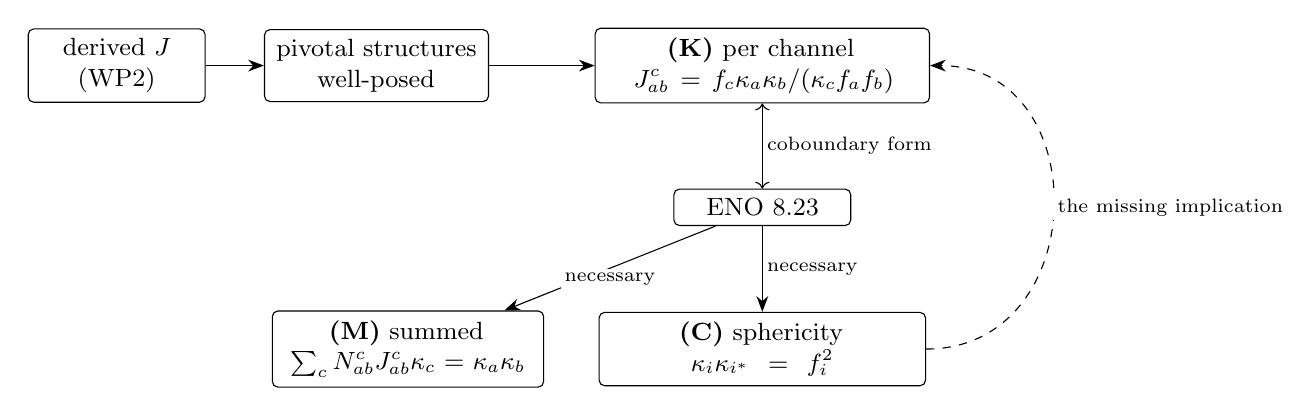
\begin{tikzpicture}[
  box/.style={draw, rounded corners=2pt, align=center, font=\small, inner sep=3.5pt},
  lab/.style={font=\scriptsize, inner sep=1.5pt, fill=white},
  ar/.style={-{Stealth[length=2mm]}, thin},
  dar/.style={-{Stealth[length=2mm]}, thin, dashed}]
\node[box, text width=2.0cm] (J) at (0.7,0) {derived $J$\\ (WP2)};
\node[box, text width=2.6cm] (piv) at (4.0,0) {pivotal structures\\ well-posed};
\node[box, text width=4.0cm] (K) at (8.9,0) {\textbf{(K)} per channel\\ $J^{c}_{ab} = f_c\kappa_a\kappa_b/(\kappa_c f_af_b)$};
\node[box, text width=2.0cm] (E) at (8.9,-1.8) {ENO 8.23};
\node[box, text width=3.9cm] (C) at (8.9,-3.6) {\textbf{(C)} sphericity\\ $\kappa_i\kappa_{i^*} = f_i^{2}$};
\node[box, text width=3.2cm] (M) at (4.4,-3.6) {\textbf{(M)} summed\\ $\sum_c N^{c}_{ab}J^{c}_{ab}\kappa_c = \kappa_a\kappa_b$};
\draw[ar] (J) -- (piv);
\draw[ar] (piv) -- (K);
\draw[ar, <->] (K) -- node[lab, right] {coboundary form} (E);
\draw[ar] (E) -- node[lab, right] {necessary} (C);
\draw[ar] (E) -- node[lab, below] {necessary} (M);
\draw[dar] (C.east) to[out=0, in=0, looseness=1.5] node[lab, right] {the missing implication} (K.east);
\end{tikzpicture}
\caption{The logical geography, corrected. (K) is the coboundary form of the target and is
equivalent to it in the signature. (C) is \emph{necessary} but not sufficient: it constrains
$\kappa$ alone, while (K) constrains $J$ on every channel, and the pointed datum
$\Vect^{\omega}_{(\Z/2)^2}$ with $J \equiv 1$ satisfies (C) and fails (K)
(\S\ref{sec:refute}). The same holds for (M), which is weaker still and is satisfied by
Yang--Lee. The dashed arrow (C)$\Rightarrow$(K) is \emph{not} a theorem of the signature; it is
part of the categorical argument that the reconstruction (WP2) and the derived twist (WP3) have
to supply. The derivation of $J$ is logically prior: it makes the other boxes statements about
determined objects.}
\label{fig:logic}
\end{figure}

Three readings of the figure matter for planning. First, \textbf{no box in it is the theorem
except (K)}, and (K) is a statement about a $J$ that has not yet been derived; the diagram is
therefore a map of obligations, not of results. Second, \textbf{(C) and (M) are necessary and
not sufficient}: each is satisfied by data on which the target fails, so neither can be used as
a lemma toward the target in the signature as it stands. Third, \textbf{the derivation of $J$
proves nothing about the target by itself}; it removes an undefined object from the statement.
This is why A2 and A3 are separate work packages and why neither can be skipped.

\subsection{The first delegation batch, and the source of truth}\label{sec:batch}

The programme begins with one reviewable batch of infrastructure and statement-settling work,
and nothing that depends on it starts until the batch has passed review. The batch:

\begin{enumerate}[label=(B\arabic*)]
\item \textbf{Reproduce the clean build} (WP0 Task~0.2): fresh clone, fresh cache, no path
override --- the ``green build'' of \S\ref{sec:prior} becomes a reproducible one, or the
reproducibility debt is diagnosed while it is still cheap.
\item \textbf{Implement the enforcing axiom audit} (WP0 Task~0.2, Gate~4 of
Appendix~\ref{app:audit}): a checked-in script that fails on Lean errors and on any dependency
outside \texttt{[propext, Classical.choice, Quot.sound]}, with a negative self-test. The
\code{\#print axioms}-plus-\code{grep} report is withdrawn.
\item \textbf{Repair the cocycle census} (WP3 Task~3.4, pulled forward): genuine cocycles in
place of the identically-trivial carry cocycle, and the two script-level witnesses
kernel-checked.
\item \textbf{Settle the corrected signature and the theorem statement} (WP1 Tasks~1.1--1.5):
the scalar contract, the qualified coherence, the carried-versus-derived distinction for $J$
(\code{derivedJ} and the \code{J_match} hypothesis of Task~2.3), and the exact target together
with its equivalence with the bare form.
\end{enumerate}

\paragraph{Source of truth.} This document, at this revision, is the source of truth for the
programme: work packages, theorem contracts, gates, and scope. The implementation-level
\texttt{PLAN.md} predates it, and this revision supersedes several of its instructions ---
among them the request for a nontrivial double-dual label permutation (withdrawn: ENO
Proposition~2.1 fixes isomorphism classes, Remark~\ref{rem:trap}) and the description of
positivity as coming from a Hermitian structure (removed: positivity is part of what ENO's
$\sigma/\tau$ argument produces, \S\ref{sec:whatdone}). Where the two documents conflict, this
proposal governs; \texttt{PLAN.md} is brought into conformance in the same revision, its
corrections are visible in the commit history, and its original step list is retained under a
superseded banner rather than rewritten. Agents delegated work on this programme are given this
paragraph verbatim.

\paragraph{Holding rule.} Dependent theorem work --- the reconstruction proofs of WP2, the
derivation of WP3 (Tasks~3.1--3.3), and the normalisation of WP4 --- does not begin until the
batch above has passed review. The rule is deliberate: every defect of \S\ref{sec:defects} was a
statement settled while proof work was already under way, and the reviews of this proposal
found the same pattern in its own instructions.

\subsection{Work packages}

The order below is the order of the schedule and of the risk: nothing in WP3--WP4 is
well-posed until WP1 has fixed the statement and WP2 has shown that the objects in it are
categorical.

\subsubsection*{WP0 --- Foundations and reproducibility (months 0--4)}

\paragraph{Objective.} Replace hand-supplied inputs with proved or explicitly labelled ones, and
make the build reproducible from a clean checkout.

\paragraph{Tasks.}
\begin{enumerate}[label=0.\arabic*]
\item Vendor the Perron--Frobenius chain (\#39914--\#39922) and define $\FPdim$ as the Perron
root of the fusion matrix; prove Theorem~\ref{thm:pf} and delete \code{FPData} where it is not
needed. Where uniqueness is genuinely required, keep the weaker \code{PFUnique} already in
\code{PFDim.lean}; otherwise \code{FPData} stays an explicit hypothesis with a per-example
certificate, and the scope statement (S\ref{sec:scope}) says so.
\item Clean-tree CI: fresh clone, \code{lake exe cache get}, \code{lake build}, and the
\emph{enforcing} audit gate of Gate~4 (Appendix~\ref{app:audit}) --- the checked-in script
\code{tools/audit-gate.sh} with its negative self-test, not the \code{\#print axioms} report
--- as separate gates, each of which fails the build. A from-clean build of the committed
tree has never been verified --- earlier builds used a path override --- and that is a
reproducibility debt no deliverable should inherit. This is also what turns the ``green build''
of \S\ref{sec:prior} into a reproducible one; it is batch item B1 (\S\ref{sec:batch}).
\item A per-file build harness with a timeout, so that a 100-second example file does not block
work on the core.
\item \code{BLUEPRINT.md} with the module dependency graph (Figure~\ref{fig:modules}), the
statement-to-source table of Appendix~\ref{app:audit} (Gate~3), and the scope labels
(S1)--(S4) attached to every theorem that depends on them.
\end{enumerate}
\paragraph{Deliverable.} D1, D2. \quad \textbf{Success criterion.} A machine with the toolchain
and no network builds the library and passes the audit from a clean clone.

\subsubsection*{WP1 --- The corrected signature and the exact target (months 1--8)}

\paragraph{Objective.} A1: make the finite-data signature express the mathematics, and make the
formal statement of the theorem say exactly what ENO and EGNO say.

\paragraph{Tasks.}
\begin{enumerate}[label=1.\arabic*]
\item \textbf{The scalar contract.} Keep the algebraic layer --- \code{FusionSystem},
\code{PivotalStructure}, the twist reduction, the census --- over a field $\field$ of
characteristic zero, where every obligation is polynomial. State the \emph{analytic} target over
$\Cx$ and only over $\Cx$: \code{ENO823Exact} is a statement about a \code{FusionSystem} over
$\Cx$ whose \code{FPData} is real ($f : \mathrm{Fin}\,n \to \R_{>0}$) embedded by
$\R \to \Cx$, whose absolute values are complex moduli, and whose positivity conjunct uses the
predicate defined in S2 --- over a general $\field$ none of these so much as typechecks, and an
earlier draft of this task asked for the target ``over a field of characteristic zero'', which
is not a meaningful contract for an analytic statement. The instances are not migrated: the
$\R$/$\Q$ ones stay, and $\Cx$-valued instances are added where the source demands them
(\S\ref{sec:scope}, S2; R5).
\item \textbf{The triangle law, derived.} The middle-unit entry
$t = F^{a\,1\,c}_{d}(a,c)$ is \emph{not} independent of the present axioms: the pentagon at
$(a,1,1,c)$ gives $t = t^{2}$, and invertibility of the associator gives $t = 1$. Prove it as a
lemma. The earlier plan to add it as a new axiom was wrong about its independence.
\item \textbf{Coherence with the nonzero-entry qualification.} The scalar coherence law may only
cancel an associator entry that is nonzero; Bartlett's Corollary~3.26 states the pivotal-symbol
coherence exactly that way. Neither support axiom supplies the qualification, and an earlier
draft of this task wrongly said they did: \code{F_support} forces zeros \emph{off} the
admissible channels and says nothing about the entries on them, and \code{J_ne_zero} is a
statement about $J$, not about $F$. So the corrected \code{J_coherent} takes one of two forms,
both acceptable: (i) the qualified law, carrying an explicit side condition
$h_F : F^{abc}_{d}(e,f) \ne 0$ at the entry to be cancelled, from which the present F-free law
follows on that channel; or (ii) the law with the $F$-factors retained,
\[
J^{e}_{ab}\, J^{d}_{ec}\, F^{abc}_{d}(e,f) \;=\; J^{f}_{bc}\, J^{d}_{af}\,
F^{abc}_{d}(e,f),
\]
from which nothing is cancelled and the F-free law is a corollary under $h_F$. The choice is
recorded in the blueprint, and WP3 proves whichever form is chosen for the derived twist. No
proof in the programme cancels an $F$-entry without an explicit nonzero hypothesis, and no
proof derives nonvanishing from \code{F_support} or \code{J_ne_zero}.
\item \textbf{Gauge-invariant duality normalisation.} Either add $\mathrm{ev}_{i^*} =
\mathrm{ev}_i$ as an axiom, or define $\dim_i = p_i\,\mathrm{coev}_i\,\mathrm{ev}_{i^*}$ as ENO
do. The first makes (K) gauge-invariant; the second matches the source but changes every instance
proof. The proposal is to do the first and prove the two normalisations agree in the self-dual
case.
\item \textbf{The exact target, and which forms are equivalent.} The library's
\code{ENO823Exact} is
\[
\code{IsPseudoUnitary}\ S \to \exists!\, P,\
P.\mathrm{IsSpherical} \wedge (\forall i,\ \dim_P i > 0) \wedge (\forall i,\ \dim_P i = f_i),
\]
which does carry existence. Every statement \emph{about} it must reproduce the existential
conjunction verbatim; the earlier rendering of the target in this proposal split it into a
spherical-structure field plus separate positivity and uniqueness fields --- asserted only
conditionally --- which is strictly weaker; it is withdrawn and is \emph{not} a proof target
(Appendix~\ref{app:statements}). What is to be proved is the equivalence of the exact form and
the \emph{bare} form \code{ENO823} ($\exists P$, spherical, $\dim_P = f$): the bare form is an
immediate consequence of the exact one, and the exact form follows from the bare one given
\code{pivotal_ext} (a pivotal structure is determined by its dimension function) and the
positivity of the FP dimensions ($\dim_P i = f_i > 0$ supplies the positivity conjunct). State
the conditional form \code{eno823_of_pseudoUnitary} separately; it assumes a pivotal structure
rather than producing one and is strictly weaker than both.
\item \textbf{The label question, recorded as closed.} Double duality fixes isomorphism classes
(ENO Proposition~2.1), so there is no label permutation to add. The plan to add one was based on
the error corrected in Remark~\ref{rem:trap}; the blueprint records the retraction and no work
item remains.
\end{enumerate}
\paragraph{Deliverables.} D3. \quad \textbf{Success criterion.} All six existing instances
re-verified under the corrected signature, with the same axiom budget; the triangle law and the
qualified coherence proved as lemmas, not assumed; a target statement that matches
Theorem~\ref{thm:eno823} field by field, stated over $\Cx$ under the scalar contract of
Task~1.1.

\subsubsection*{WP2 --- Reconstruction and the trace correspondence (months 3--10)}

\paragraph{Objective.} Make the words in the statement mean what they say. Until the skeletal
datum is a category, ``the categorical dimension'' is a scalar defined by a formula, and the
theorem is a statement about a formal system.

\paragraph{Tasks.}
\begin{enumerate}[label=2.\arabic*]
\item \textbf{A small reconstruction.} For multiplicity-free data, define the $\field$-linear
category whose objects are formal finite direct sums of simples and whose morphisms are matrices
indexed by channels; prove it is monoidal, rigid, semisimple, and that $\mathrm{End}(\one) =
\field$. The associativity and unit constraints are the $F$-data and the unit laws; the snakes
are the snake axioms. This is the piece of the programme that converts a formal calculation into
a theorem about fusion categories, and it is scheduled before the twist because the twist is a
morphism of the reconstructed category.
\item \textbf{The trace correspondence.} Prove that the categorical trace of $p_i \colon X_i \to
X_i^{**}$ is $p_i \kappa_i$, that $\mathrm{Tr}(a_i) = a_i\,\mathrm{coev}_i\,\mathrm{ev}_{i^*}$
is ENO's $d_i$, and that $\kappa_i \kappa_{i^*} = |X_i|^{2}$ in the sense of
Definition~\ref{def:pseudo}. This is small, checkable, and closes the gap between the library's
scalars and the source's dimensions.
\item \textbf{The twist as a morphism: derived $J$, and its relation to the carried field.}
From the reconstructed category, \emph{define} \code{derivedJ} as the scalar of the
monoidal structure of $(-)^{**}$ on the channel $(i,j;k)$ --- i.e.\ a specific morphism
$X_i^{**} \otimes X_j^{**} \to (X_i \otimes X_j)^{**}$ --- so that WP3 derives a morphism and
not a table. Do \emph{not} identify \code{derivedJ} with the datum's carried field $S.J$: that
field is free data constrained only by the four twist laws, and the pointed false-$J$ datum
($\Vect^{\omega}_{(\Z/2)^{2}}$ with $J \equiv 1$, \S\ref{sec:refute}) satisfies every law the
signature imposes while its honest tensorator is $\delta(\kappa)$. The relation between the
two is therefore an explicit \emph{compatibility hypothesis}, \code{J_match}, stating that
$S.J$ and \code{derivedJ} agree on every channel, discharged per instance by WP3 (Task~3.3),
or else the corrected signature of WP1 replaces the carried field by the derived definition
once WP3 has proved the four laws for it. Reconstruction must not ask for the identification
outright: that instruction is contradicted by the false-$J$ example, and an earlier draft of
this task gave it.
\end{enumerate}
\paragraph{Deliverables.} D4. \quad \textbf{Success criterion.} The reconstructed category is a
\code{FusionCategory} in the sense of the library's own definition, and every scalar named in
the target is the corresponding trace; \code{derivedJ} is defined independently of the carried
field, and the relation between the two is the explicit hypothesis \code{J_match} or a field
replacement --- never an identification by fiat.

\subsubsection*{WP3 --- Deriving the double-dual twist (months 4--14)}

\paragraph{Objective.} A2: $J$ as a function of $(F, \mathrm{ev}, \mathrm{coev})$, derived and
not transcribed.

\paragraph{The retraction this package has to respect.} \texttt{PLAN.md} records that the
displayed formula
\[
\Omega(a,b;c) = F^{b^*a^*c}_{0}(c^*,b)\cdot (M_b)^{-1}(0,c)
\]
is \emph{defective as written}: read literally it returns $+1$ on $(\Z/2)^2$ with
$\omega = (-1)^{a_1b_2c_1}$, where the honest twist is $\delta(\kappa)$, i.e.\ $-1$ on six
channels. The construction of the comparison is right and the transcription is not.
\code{docs/honest\_twist\_check.py} evaluates the twist from its defining property and never
evaluates the displayed $\Omega$. No milestone below depends on the displayed formula.

\paragraph{Tasks.}
\begin{enumerate}[label=3.\arabic*]
\item \textbf{The comparison map.} Construct $\psi_{a,b} \colon \dual{(a \otimes b)} \to \dual b
\otimes \dual a$ as the unique map intertwining the evaluations, and prove it is an isomorphism.
\item \textbf{The ratio formula.} Prove
\[
J^{c}_{ab} \;=\; \frac{\psi_{a,b}|_{c}}{\psi_{b^*,a^*}|_{c^*}},
\]
and \emph{then} derive a closed form in terms of $F$; if the closed form differs from the
retracted $\Omega$, the retraction is the correct record and the new formula replaces it in
\texttt{PLAN.md} and the blueprint.
\item \textbf{The four laws and the qualified coherence} of WP1 Task~1.3, proved for the
derived twist \code{derivedJ} of WP2 Task~2.3. This is the step that
turns ``$J$ is data'' into ``$J$ is computed'', and it is independent of pseudo-unitarity. For
instances carrying their own $J$ field, the compatibility hypothesis \code{J_match} of
Task~2.3 is discharged here; alternatively the corrected signature of WP1 replaces the carried
field by \code{derivedJ}, in which case there is nothing to match.
\item \textbf{Repair the census.} The cyclic families in \code{docs/pointed\_twist\_check.py} use
a ``carry cocycle'' whose exponent is a multiple of $n$, so it is identically $1$, and for cyclic
groups $\kappa$ is a character, so those cases cannot separate the honest twist from the trivial
one (\S\ref{sec:refute}). Replace them with genuine cocycles: $(\Z/2)^2$, $(\Z/3)^2$, a
non-trivial $3$-cocycle on $\Z/3$, and a non-abelian group; kernel-check the two witnesses that
are currently script-level.
\item \textbf{Independent confirmation.} Compare index by index with Bartlett's Theorem~4.17 and
Corollary~3.26, and with the corrected census. A mismatch is a defect in the derivation, not in
the check.
\item \textbf{(M) as an acceptance test.} For the genuine $J$, (M) should be a theorem --- the
dimension of a pivotal category is multiplicative. A failure of (M) after the derivation means
the derivation is wrong; it is not evidence that (M) is an extra hypothesis.
\end{enumerate}
\paragraph{Deliverables.} D5. \quad \textbf{Success criterion.} The library contains no
hypothesis on $J$ beyond the four laws; they are theorems about the derived object; the census
contains at least four genuinely non-trivial cocycles and is kernel-checked. \textbf{Explicit
non-goal:} WP3 does not prove (K). The target is the strictly stronger per-channel identity,
which fails for Yang--Lee and is WP4's content.

\subsubsection*{WP4 --- ENO's normalisation and the theorem (months 8--20)}\label{sec:wp4}

\paragraph{Objective.} A3: ENO~8.23, with the normalisation argument stated as ENO state it.

\paragraph{Tasks.}
\begin{enumerate}[label=4.\arabic*]
\item \textbf{Construct $a$.} An additive isomorphism $a \colon \Id \to (-)^{**}$ with $a^{2} =
g$ monoidal. \code{SqrtData} currently assumes $a$; this task constructs it from $g$
(Theorem~\ref{thm:quad}), which is either a hypothesis (S3, first option) or a theorem of WP4
Task~4.2.
\item \textbf{The quadruple dual.} Either keep $g$ as an explicit hypothesis, or formalise
Bartlett's Theorem~3.28 and Corollary~3.30: the quadruple-dual functor is monoidally isomorphic
to the identity, proved by string diagrams (\S3.6 of \cite{Bartlett1502}) and avoiding the weak
Hopf algebra theory of ENO \S4--5. This is the single largest prerequisite in the programme and
is budgeted as such; if it slips, the theorem is stated conditionally.
\item \textbf{The bound.} From the trace identity $d_i d_j = \sum_c T^{ij}_c d_c$ with
$T^{ij}_c = N^{ij}_c b^{ij}_c$ and $|b| = 1$, derive $|d_i| \le f_i$ by ENO's weighted norm. The
library has the weighted-norm argument (\code{abs_le_fpdim_of_eigenvector}); what is missing is
the passage from the $T$-matrix to the $N$-matrix, i.e.\ the triangle inequality
$|\sum_j T^{ik}_j d_j| \le \sum_j N^{ik}_j |d_j|$.
\item \textbf{The sum identity.} Prove $\sum_i |d_i|^{2} = \dim \C$ for $d_i = a_i \kappa'_i$,
which under pseudo-unitarity gives $\sum_i |d_i|^{2} = \sum_i f_i^{2}$; the equality case of
Theorem~\ref{thm:821} then yields $|d_i| = f_i$.
\item \textbf{The two normalisations, correctly typed.} This is the step the earlier draft of this
proposal misstated, and it is worth stating exactly.
  \begin{enumerate}[label=(\alph*)]
  \item The chain $f_i f_j = |d_i d_j| \le \sum_c N^{c}_{ij} f_c = f_i f_j$ is an equality; hence
  $T^{c}_{ij} = \pm N^{c}_{ij}$ and $d_i d_j/d_c$ is real whenever $N^{c}_{ij} > 0$. Consequently
  $\sigma_i = d_i^{2}/|d_i|^{2}$ defines a \emph{tensor automorphism of the identity functor}.
  It is not sign-valued a priori --- it is a phase --- and its monoidality is exactly a
  statement about \emph{squares}: on every channel,
  \[
  (d_i d_j/d_c)^{2} \;=\; (f_i f_j / f_c)^{2} \;>\; 0 ,
  \]
  so only the squares of the ratios are pinned down and positive at this stage; the ratios
  themselves are real of fixed modulus and undetermined sign, and fixing the signs is precisely
  the work of the $\tau$-step below. (An earlier draft of this task said the ratios themselves
  were positive here; that presupposes the $\tau$-step and is corrected.)
  \item Twisting $g$ by $\sigma$ makes the new dimensions real. After this, $\tau_i = d_i/|d_i|$
  is $\pm 1$; it is a \emph{natural} automorphism, not a monoidal one, and it is applied to $a$,
  not to $g$.
  \item After the $\tau$-twist, $T = N$ and $b = 1$, so $a$ is a pivotal structure with
  $\dim = f > 0$.
  \end{enumerate}
  The point to keep: multiplying $a$ by a monoidal character leaves the defect
  $b^{ij}_{c} = J^{ij}_{c} a_i a_j/a_c$ \emph{unchanged}, so the $\sigma$-step cannot remove a
  defect; it normalises the phase. The $\tau$-step is the one that acts on $a$, and it is not
  monoidal. A draft that made both steps ``tensor autoequivalences acting by signs'' was wrong on
  both counts. (For a concrete illustration: in $\Vect_{\Z/3}$ the tuple $a = (1,-1,1)$ satisfies
  $a^{2} = 1 = g$ but is not a character, so rescaling a square root by arbitrary scalars changes
  the defect.)
\item \textbf{Assembly and uniqueness.} \code{eno823\_exact}: existence, positivity, equality with
$\FPdim$, uniqueness via \code{pivotal\_ext} and \code{PFUnique}.
\end{enumerate}
\paragraph{Deliverables.} D6. \quad \textbf{Success criterion.} \code{ENO823Exact} proved for
multiplicity-free data over $\Cx$ under the scalar contract of WP1 Task~1.1, with the
hypothesis on $g$ either
discharged (Bartlett route) or explicitly labelled; \code{YangLee.not\_pseudoUnitary} as the
sharpness witness.

\subsubsection*{WP5 --- Cover, grading, and the frontier (months 14--22, off the critical path)}\label{sec:wp5}

\paragraph{Objective.} A4: the part of the theory that does not need pseudo-unitarity, stated
precisely enough to be useful and no more.

\paragraph{Tasks.}
\begin{enumerate}[label=5.\arabic*]
\item \textbf{The cover as an equivariantization.} Bartlett \S5.3: the sphericalization
$\widetilde{\C}$ is the equivariantization of $\C$ with respect to the canonical $\Z/2$-action,
\emph{not} a $\Z/2$-graded extension of $\C$. Prove it is a fusion category, identify the
forgetful functor, and prove $\dim \widetilde{\C} = 2\dim \C$. The present \code{Cover.lean} is
scaffolding: \code{coverGlobalDim\_double} is a reindexing identity and
\code{coverCanonicalPivotal} returns a scalar with no \code{PivotalStructure}.
\item \textbf{The torsor.} Given one pivotal structure, the set of pivotal structures is a torsor
under $\mathrm{Hom}(U_{\C}, \field^{\times})$, where $U_{\C}$ is the universal grading group.
This is a statement about \emph{differences} between existing structures.
\item \textbf{What is withdrawn.} The draft claimed the criterion
\[
\mathrm{Pivotal}(\C) \neq \varnothing \iff [g] \text{ is a square in }
\mathrm{Hom}(U_{\C}, \field^{\times}),
\]
and the corollary that $\C$ is pivotal when $U_{\C}$ has no $2$-torsion. Neither is available.
A map $g \colon \Id \to (-)^{****}$ is not an automorphism of $\Id$, so its class is not a
character class without an identification the project does not have; and the criterion fails even
for monoidal $g$: $\Vect_{\Z/2}$ with $g$ the non-trivial character is pivotal, while that
character has no square root in $\mathrm{Hom}(\Z/2, \Cx)$. A torsor does not establish existence.
Any replacement needs a precise source and a separate proof, and is not promised.
\end{enumerate}
\paragraph{Deliverables.} D7. \quad \textbf{Success criterion.} The cover is a
\code{FusionSystem} with a \code{PivotalStructure} and is described as an equivariantization; the
torsor statement is proved for differences; no existence criterion is stated.

\subsubsection*{WP6 --- The categorical bridge and upstream (months 12--24)}

\paragraph{Objective.} Mathlib's categorical definitions become the ones the library uses, and
the vendored placeholders disappear.

\paragraph{Tasks.}
\begin{enumerate}[label=6.\arabic*]
\item \textbf{The pivotal equivalence.} On the category of WP2, prove
$\mathrm{PivotalStructure}\ S \simeq \mathrm{PivotalCategory}\ (\mathrm{CategoryOf}\ S)$: Mathlib's
monoidal natural isomorphism $\mathrm{Id} \to (-)^{**}$ restricts to the scalars $p_i$ and
\code{p\_mon} is its coherence.
\item \textbf{Delete the placeholders.} When \#42145/\#42150/\#42191 merge, replace
\code{PivotalCategory.lean} by an import. Until then the file declares nothing used elsewhere, and
the blueprint says so.
\item \textbf{Contribute back.} The Perron--Frobenius material and the spherical layer are the
two pieces of independent upstream value.
\end{enumerate}
\paragraph{Deliverables.} D8. \quad \textbf{Success criterion.} \code{MathlibPatches/} contains
no mathematics, only imports.

\subsubsection*{WP7 --- Instances, witnesses, and the regression suite (continuous)}

\paragraph{Objective.} Every theorem in the library has an inhabitant, and every defect in
the table of \S\ref{sec:defects} has a regression test.

\paragraph{Tasks.}
\begin{enumerate}[label=7.\arabic*]
\item Extend the instance set, over $\Cx$ as well as $\R$: $\Vect^{\omega}_{\Z/n}$ for
$n = 2,\dots,6$ with genuine cocycles; Tambara--Yamagami for $\Z/2$; the rank-three ring
$K(1,0,1)$ already present; $H_3$ (non-integer $\FPdim$) as a test that nothing assumes
integrality.
\item Formalise the two script-level witnesses of \S\ref{sec:refute}:
$\Vect^{\omega}_{(\Z/2)^2}$ with $J \equiv 1$ (the failure of (M)) and
$\Vect^{\omega}_{(\Z/3)^2}$ (the failure of $J^{2} = 1$).
\item A \emph{negative} multiplicity test. The based ring $X^{2} = \one + 2X$ is legitimate, but
it has no fusion-category categorification over $\Cx$ (\cite{OstrikRank2}, Theorem~2.1). It is used to test
the indexing of a matrix-valued associator and as a negative example against any claim that a
based ring categorifies; it cannot supply a coherent rigid witness, and no such witness for
$N = 2$ is promised by this programme.
\item A census harness with genuine cocycles, failing the build on disagreement with the reference
computations.
\end{enumerate}
\paragraph{Deliverables.} D9. \quad \textbf{Success criterion.} Sixteen data sets, at most two of
them script-only, at least four with genuinely non-trivial cocycles, and the census harness green.

\subsection{Milestones}

\begin{center}
\small
\begin{tabularx}{\textwidth}{@{}l>{\raggedright\arraybackslash}p{0.27\textwidth}Ll@{}}
\toprule
\textbf{Milestone} & \textbf{Month} & \textbf{Content} & \textbf{Deliverable} \\
\midrule
M0 & 2 & First delegation batch passed review: reproduced clean build; enforcing audit gate green with its self-test; census repaired; signature and exact target settled & D2 (part) \\
M1 & 4 & \code{FPData} proved or labelled; clean-tree CI with the enforcing audit gate; blueprint with the statement-to-source table & D1, D2 \\
M2 & 8 & Signature v2 (the $\Cx$ scalar contract, triangle derived, qualified coherence, gauge fix); \emph{exact} target; six instances re-verified & D3 \\
M3 & 10 & Reconstruction and trace correspondence; $J$ identified as a morphism & D4 \\
M4 & 14 & $J$ derived; four laws and qualified coherence proved; census repaired and kernel-checked & D5 \\
M5 & 18 & $a$ constructed; $T$-matrix domination; bound $|d_i| \le f_i$; sum identity and equality case & D6 (part) \\
M6 & 20 & $\sigma$ (tensor) and $\tau$ (natural) normalisations; \code{ENO823Exact} proved & D6 \\
M7 & 22 & Cover as equivariantization; torsor for differences; withdrawn criterion recorded & D7 \\
M8 & 24 & Bridge to \code{PivotalCategory}; placeholders deleted; release v1.0; papers submitted & D8, D10--D12 \\
\bottomrule
\end{tabularx}
\end{center}

\section{Techniques}\label{sec:techniques}

\subsection{Finite data and exact arithmetic}

Everything categorical is reduced to finite algebra over a field, and everything numeric is done
exactly. Two devices carry the instances.

\paragraph{Integer pairs in $\Z[\sqrt d]$.} Real numbers never appear in a proof obligation.
Each entry of $F$, $\mathrm{ev}$, $\mathrm{coev}$, $J$ in the Fibonacci, Ising and Yang--Lee
examples is an integer pair $(p,q)$ denoting $(p + q\sqrt d)/2$ in $\Q(\sqrt d)$; the field
operations are defined on pairs, and \code{decide} checks the pentagon, the unit laws, the
inverse laws and the snakes on all label tuples. For Ising, $d = 2$ and the scalar $1/\sqrt2$
enters as a normalisation, so the identities are checked twice --- once for the rational part
and once for the $\sqrt2$ part. This is why the examples are trustworthy despite being
numerical, and it is why they compile in 100 seconds rather than hours.

\paragraph{Field checks are hand-written.} Closing real-number arithmetic is not automatic:
\code{one_lt_pow} and its primed variant were unusable in the Yang--Lee file, and the
$\varphi^{4}$ contradiction had to be assembled by hand from \code{nlinarith} with an explicit
$\sqrt5 \cdot \sqrt5 = 5$. A mis-stated closed form for $((1+\sqrt5)/2)^{2}$ cost a build cycle.
The practical rule adopted is: get the closed form right on paper, then prove it once, then
reuse.

\subsection{Inhabitant-first statement design}\label{sec:tech-inhabitant}

The four defects of \S\ref{sec:prelim} share one cause: a statement was written to look like its
source and then trusted. The remedy, now institutionalised in this project, is that \emph{no
statement is committed until an inhabitant exists}, and no axiom is believed until an example
satisfies it and a non-example does not. Concretely:

\begin{enumerate}[label=(\roman*)]
\item every structure gets a witness in the same commit as its definition
(\code{VecZ2.system} with the definition of \code{FusionSystem});
\item every axiom gets a regression test that fails if the axiom is strengthened
(\code{swapped_Finv_comp_ne_one} for the snake; \code{VecZ2Twisted} for the twist);
\item every theorem whose statement mentions a hypothesis gets a witness that the hypothesis is
needed (Yang--Lee for positivity; $\Vect^{\omega}_{(\Z/2)^2}$ for multiplicativity).
\end{enumerate}

The cost is real --- the witness files are about half the library --- and it is the single
highest-value investment in the programme, because the defects it catches are exactly the ones
that survive refereeing.

\subsection{Falsification before proof}\label{sec:tech-falsify}

For each proposed statement $S$, the programme first looks for a counterexample, in this order:
(i) on paper, on the smallest rank; (ii) in Python, on the full data set, with the associators
composed as matrices rather than manipulated symbolically; (iii) in Lean, by attempting the
statement on the counterexample candidate before attempting the theorem.

This order is not a heuristic. Two of the project's four defects were found this way, and a
third --- the `$J \equiv 1$` claim for pointed categories --- was refuted by an exhaustive
computation in \code{docs/pointed_twist_check.py} after it had been stated in the plan. The
Python step matters because matrix composition over channel bases is where index conventions
break, and because a script that recomputes every scalar from the snake axioms is an independent
implementation, not a restatement.

\subsection{Multiplicities: why this is a separate development}\label{sec:tech-mult}

With $N^{k}_{ij} > 1$ the Hom space $\mathrm{Hom}(X_k, X_i \otimes X_j)$ has dimension $N^{k}_{ij}$
and the associator at fixed $(a,b,c,d)$ is a matrix whose entries are themselves matrices; the
pentagon becomes a matrix identity with channel bases on both sides, and ``the'' $F$-symbol is a
choice of bases. Three consequences:

\begin{enumerate}[label=(\roman*)]
\item the scalar signature cannot be extended by adding a parameter --- the type of \code{F}
changes, and every instance proof that ends in \code{decide} over \code{Fin n} must be rewritten;
\item gauge freedom is larger (a $\mathrm{GL}_{N}$-valued change of channel bases); the twist
$J$ becomes an operator between multiplicity spaces, and the condition it satisfies ---
multiplicativity, or the per-channel identity --- is an \emph{operator equality on each
multiplicity space}, not a scalar equation. Taking a determinant or a trace of that equality
destroys the monoidality information and does not give the scalar law: the general statement has
no scalar reformulation of the kind the multiplicity-free case has;
\item the correct target in the general case is the \emph{categorical} statement (WP6), with the
skeletal statement as a corollary in the multiplicity-free case.
\end{enumerate}

The proposal therefore treats the multiplicity-free theorem as the deliverable and the general
case as a stretch goal, pursued through the categorical bridge rather than through a bigger
scalar signature. This is a scope decision, stated here so that it can be argued with.

\subsection{Diagram evaluation and independent reference computations}

The one place where the project has repeatedly gone wrong is the evaluation of a diagram with
more than two $F$-moves. The technique that works is to evaluate the same diagram twice by
different routes:

\begin{itemize}
\item an \emph{evaluation-side} assembly (compose evaluations, transport coevaluations);
\item a \emph{coevaluation-side} assembly;
\item the $\Omega$-coefficient form of WP2 Task 2.2;
\item the direct $\varphi$-evaluation from its defining property
$\mathrm{ev} \circ (\varphi \otimes \mathrm{id}) = \mathrm{ev}$, with full associator
bookkeeping (\code{docs/honest_twist_check.py}).
\end{itemize}
Agreement of four independent assemblies on sixteen data sets is the current standard of evidence
for a formula, and it is what caught the defective transcription of $\Omega$ recorded in the
plan. It is \emph{not} a proof, and the proposal does not treat it as one: the kernel proof of
WP2 Task 2.3 is what settles the formula, and the scripts are demoted to regression tests.

A second, independent technique is the Temperley--Lieb check: in $\mathrm{TL}(\varphi)$ one can
compute the loop scalar of Fibonacci with no $F$-data at all, and it gives $\kappa_\tau =
\varphi$ against the naive $\varphi^{2}$. It certifies the snake normalisation and nothing else,
which is exactly the scope claimed for it.

\subsection{Parallel adversarial exploration}

The project uses a workbench in which several agents attack one problem in independent
directions, register their direction on a shared board, and submit reports that a coordinating
agent accepts only after re-deriving or kernel-checking the claim. Two things are worth
recording, because both bear on the proposed programme.

\paragraph{What it bought.} The pointed-case value of the twist, $J = \delta(\kappa) =
\kappa_a\kappa_b/\kappa_c$, was settled in this mode by three independent assemblies; the
identification of the trace identity with (M) emerged from it; and four independent evaluations
of the $J$-diagram agreed, which is what isolated the defective $\Omega$ transcription.

\paragraph{What it got wrong.} The same mode produced claims that did not survive checking: that
$X^{**} \cong X$ canonically in any rigid monoidal category (false --- this is precisely
pivotality, and adopting it would have made the signature vacuous, as it had already done once);
a scalar formula for $\psi$ that returns $1$ on channels where the honest twist is $-1$; and the
assertion $J \equiv 1$ for pointed categories, which is false and was replaced by
$\delta(\kappa)$. Each was caught by the acceptance rule, not by the generating agents.

\paragraph{Consequence for the programme.} The technique is used for exploration and for
independent assembly, never as evidence. Every claim in \S\ref{sec:prelim} marked ``kernel'' has
been re-proved or re-checked by the coordinating agent; claims marked ``script'' are labelled as
such; and no report is merged on the strength of its own text. The proposal's WP3 and WP4
explicitly budget for this: parallel exploration of the positivity step and of the cover, with
kernel acceptance.

\subsection{Statement fidelity as a method}\label{sec:fidelity}

The four defects are instances of four general failure modes, and naming them is part of the
proposed contribution.

\begin{enumerate}[label=\textbf{F\arabic*.},leftmargin=2.4em]
\item \textbf{Vacuity.} The hypothesis is inconsistent, so the theorem is true and empty. Detected
by inhabitation, not by proof.
\item \textbf{Drift.} The formal statement is a different, usually stronger, statement (a
one-line axiom where the source has a coherence condition). Detected by proving the source's
examples fail, or by checking that the statement is not provable without its hypothesis.
\item \textbf{Unrepresentability.} The signature cannot express the general case (real scalars
where the source is complex; no multiplicity). Detected by trying to state the general theorem,
not by proving the special one. Note that the label question is \emph{not} an instance: double
duality always fixes isomorphism classes (ENO Proposition~2.1), and an earlier draft of this
proposal wrongly listed $i^{**} \neq i$ here.
\item \textbf{Normalisation.} The statement is right but the gauge is wrong: a reciprocal where a
matrix inverse is required, a sign convention that excludes the examples. Detected by the
examples, and only by the examples.
\end{enumerate}

The audit protocol that follows is mechanical and is written up in Appendix~\ref{app:audit}. It
has three gates: \emph{inhabitation} (does the structure have a witness?), \emph{sharpness} (is
the hypothesis used, i.e.\ does dropping it admit a counterexample?), and \emph{correspondence}
(is the statement the source's, with its numbering and its quantifiers?). The third gate is the
one a proof assistant cannot automate, and the one that caught D3.

\subsection{Engineering discipline}

\begin{itemize}
\item \textbf{Pinned toolchain.} Lean \texttt{v4.33.1}, Mathlib \texttt{0df444a3}, in both
packages; no bump without updating both lockfiles.
\item \textbf{No \texttt{sorry}, no \texttt{axiom}}, axiom budget
\texttt{[propext, Classical.choice, Quot.sound]} enforced by the audit gate of Gate~4
(Appendix~\ref{app:audit}) --- a script that fails the build on Lean errors and on
out-of-budget dependencies, self-tested against a deliberate \texttt{sorry}. The printed
\code{AxiomAudit.lean} report alone enforces nothing.
\item \textbf{Per-file builds} with generous timeouts (an \code{import Mathlib} costs 20--60
seconds; the example files cost minutes), \code{weakLeanArgs = ["-j2","-s8192"]} to stay inside
CI memory limits.
\item \textbf{No module-private declarations}: the project avoids the bare \code{module} header,
which makes declarations private and breaks downstream imports in a way that is hard to diagnose.
\item \textbf{Commit messages as a proof log}, including retractions. The repository's history
carries three commits whose subject is a correction of the previous commit's mathematics; that
is a feature, and the plan keeps the record rather than rewriting it.
\end{itemize}
\section{Risks and mitigations}\label{sec:risk}

The risk of this programme is not concentrated in the analysis. It is concentrated in
\emph{statement correctness} and \emph{reconstruction}: the preliminary work got four statements
wrong before getting them right, and the analytic step cannot even be stated until the skeletal
datum is a category. The table makes the dependencies explicit, in the order in which they bite.

{\small
\begin{longtable}{@{}>{\raggedright\arraybackslash}p{0.05\textwidth}>{\raggedright\arraybackslash}p{0.29\textwidth}>{\raggedright\arraybackslash}p{0.50\textwidth}>{\raggedright\arraybackslash}p{0.08\textwidth}@{}}
\toprule
& \textbf{Risk} & \textbf{Mitigation / fallback} & \textbf{Level} \\
\midrule
\endfirsthead
\toprule
& \textbf{Risk} & \textbf{Mitigation / fallback} & \textbf{Level} \\
\midrule
\endhead
\bottomrule
\endlastfoot
R1 & \textbf{Statement correctness.} A work package targets a statement that is not the
source's, or a normalisation that is wrong. Four instances already occurred in the preliminary
work, and an external reading of the first draft of this proposal found six more. & Gate~3 of Appendix~\ref{app:audit}: every
theorem carries its source, edition, numbering and quantifiers; the exact target is reproduced
verbatim; two independent readings of each new statement before it is scheduled. & high \\
R2 & \textbf{Reconstruction.} The skeletal datum may not reconstruct as a fusion category from the
present axioms, and the reconstruction is real category theory inside Mathlib. & WP2 does the
multiplicity-free case first and is scheduled early; fallback: every theorem is labelled
``skeletal'' rather than ``categorical'' and the categorical claim is withdrawn from the abstract.
& med/high \\
R3 & \textbf{The twist derivation.} No correct closed form is known; the $\Omega$ formula in
\texttt{PLAN.md} is retracted, and the census that appeared to support it is inconclusive. &
Derive through the comparison $\psi$, kernel-check, and cross-check against Bartlett's
Theorem~4.17 and Corollary~3.26; fallback: keep $J$ a hypothesis and state the theorem
conditionally on it. & med/high \\
R4 & \textbf{The quadruple dual.} ENO Theorem~2.6 needs weak Hopf algebras, out of scope;
Bartlett's graphical proof is the alternative and is a large formalisation. & Budgeted as a
separate task with its own deliverable; fallback is the conditional statement, labelled. & med \\
R5 & \textbf{Complex scalars.} The library is over $\R$; $\Cx$ breaks the \code{decide}-based
instance proofs, which use integer pairs in $\Z[\sqrt d]$. & Model $\Q(\zeta)$ by integer
polynomials mod $\Phi_n$ and keep \code{decide} exact; keep the $\R$ instances and add $\Cx$ ones
rather than migrating. & med \\
R6 & \textbf{The normalisation step.} ENO's $\sigma/\tau$ argument needs the operator-level
multiplicativity that WP2 supplies; if the reconstruction slips, this is unavailable. & The
conditional theorem \code{eno823_of_pseudoUnitary} already isolates the gap; publish the
conditional result if necessary. & med \\
R7 & Mathlib churn: \#42150/\#42191 merge with different names, or stall. & Vendor, keep
byte-compatible, switch by replacing one import; contribute the spherical layer if it stalls. &
low \\
R8 & Elaboration cost: \code{decide} over $3^{n}$ label tuples grows fast; example files already
cost 100\,s. & Exact arithmetic in $\Z[\sqrt d]$; per-file builds; abstraction barriers so the
core does not import the examples; \texttt{native\_decide} forbidden. & low \\
R9 & \textbf{Scope.} A single investigator over 24 months, on a theorem whose unconditional form
exceeds the plan. & The scope statement (S\ref{sec:scope}) is part of every deliverable; D1--D6
are the core and D7--D12 are additive; WP5 is off the critical path. & med \\
\end{longtable}
}

\paragraph{The stop conditions.} Two, and they are decided at fixed months rather than at the
end. If by month 12 the reconstruction of WP2 has not produced a category, the programme drops
the categorical claim and publishes the skeletal theorem as such. If by month 16 the twist
derivation of WP3 has not succeeded, the theorem is stated with $J$ as an explicit hypothesis,
and the deliverable is the conditional result together with the Yang--Lee sharpness theorem.
Neither outcome is a failure; both must be decided on time.

\section{Timeline}\label{sec:timeline}

Twenty-four months, eight quarters. Bars mark active work. The order is forced by the
dependencies: signature and exact target (WP1), then the reconstruction that makes the words
mean something (WP2), then the twist (WP3), then ENO's normalisation (WP4). The cover and grading
work (WP5) is deliberately late and off the critical path, because its statements are the ones
most in need of justification.

\begin{center}
\small
\begin{tabular}{@{}l*{8}{c}@{}}
\toprule
\textbf{Work package} & \textbf{Q1} & \textbf{Q2} & \textbf{Q3} & \textbf{Q4} &
\textbf{Q5} & \textbf{Q6} & \textbf{Q7} & \textbf{Q8} \\
\midrule
WP0 Foundations & $\blacksquare$ & $\blacksquare$ & & & & & & \\
WP1 Signature \& exact target & $\blacksquare$ & $\blacksquare$ & $\blacksquare$ & & & & & \\
WP2 Reconstruction \& trace & & $\blacksquare$ & $\blacksquare$ & $\blacksquare$ & & & & \\
WP3 Derived twist & & $\blacksquare$ & $\blacksquare$ & $\blacksquare$ & $\blacksquare$ & & & \\
WP4 ENO normalisation \& theorem & & & $\blacksquare$ & $\blacksquare$ & $\blacksquare$ & $\blacksquare$ & $\blacksquare$ & \\
WP5 Cover \& grading & & & & & $\blacksquare$ & $\blacksquare$ & $\blacksquare$ & $\blacksquare$ \\
WP6 Bridge \& upstream & & & & & $\blacksquare$ & $\blacksquare$ & $\blacksquare$ & $\blacksquare$ \\
WP7 Instances \& tests & $\blacksquare$ & $\blacksquare$ & $\blacksquare$ & $\blacksquare$ & $\blacksquare$ & $\blacksquare$ & $\blacksquare$ & $\blacksquare$ \\
\midrule
\emph{Milestones} & M0 & M1 & M2 & M3 & M4 & M5 & M6, M7, M8 \\
\bottomrule
\end{tabular}
\end{center}

\section{Expected deliverables}\label{sec:deliverables}

Twelve deliverables, each with a month and an acceptance criterion. D1--D6 are the core; D7--D12
are additive and independently valuable. The scope labels (S1)--(S4) of \S\ref{sec:scope}
apply to every deliverable below, and the conditional and unconditional forms of the theorem are
listed separately.

{\small
\begin{longtable}{@{}>{\raggedright\arraybackslash}p{0.045\textwidth}>{\raggedright\arraybackslash}p{0.29\textwidth}>{\raggedright\arraybackslash}p{0.52\textwidth}>{\raggedright\arraybackslash}p{0.085\textwidth}@{}}
\toprule
& \textbf{Deliverable} & \textbf{Acceptance criterion} & \textbf{Month} \\
\midrule
\endfirsthead
\toprule
& \textbf{Deliverable} & \textbf{Acceptance criterion} & \textbf{Month} \\
\midrule
\endhead
\bottomrule
\endlastfoot
D1 & \textbf{Core library v1.0}: fusion rings; Perron--Frobenius dimension with \code{FPData}
proved or explicitly labelled; skeletal systems; pivotal and spherical layers; the twist
reduction; ENO 8.21. & Reproducible clean build; no \texttt{sorry}; every audited declaration at
\texttt{[propext, Classical.choice, Quot.sound]}. & 4--20 \\
D2 & \textbf{Reproducibility kit}: pinned toolchain, CI gates, clean-tree script, per-file
harness, archived artifact with a DOI. & A fresh clone builds and audits without manual steps;
the difference from the working-tree build is documented. & 4 \\
D3 & \textbf{Corrected signature and exact target}: the $\Cx$ scalar contract; triangle law
derived; coherence with the nonzero-entry qualification (explicit nonzero side condition or
retained $F$-factors); gauge-invariant duality normalisation; the target
matching ENO 8.23 / EGNO 9.5.1 field by field. & All six existing instances re-verified; the new
lemmas proved, not assumed; the target's existential conjunction reproduced verbatim, stated
over $\Cx$ with FP dimensions embedded from $\R$. & 8 \\
D4 & \textbf{Reconstruction and trace correspondence}: the multiplicity-free datum is a fusion
category; every scalar in the target is the corresponding categorical trace; $J$ identified as a
morphism. & The reconstructed category satisfies the library's own \code{FusionCategory}
predicate, and the trace identities are theorems. & 10 \\
D5 & \textbf{Derived twist}: the comparison $\psi$, the ratio formula, the four laws, the
qualified coherence, a repaired census with genuine cocycles, and the Bartlett comparison. & No
hypothesis on $J$ remains; at least four genuinely non-trivial cocycles, kernel-checked; the
retracted $\Omega$ either corrected or replaced in \texttt{PLAN.md}. & 14 \\
D6 & \textbf{ENO 8.23}: $a$ constructed, $T$-matrix domination, the bound $|d_i| \le f_i$, the
sum identity, the $\sigma/\tau$ normalisation, uniqueness. & \code{ENO823Exact} proved for
multiplicity-free data over $\Cx$ under the scalar contract of WP1 Task~1.1; the hypothesis on
$g$ either discharged
(Bartlett) or explicitly labelled. & 20 \\
D7 & \textbf{Cover and torsor}: the cover as an equivariantization, with doubled dimension; the
torsor for differences of pivotal structures; the withdrawn existence criterion recorded. & The
cover is a \code{FusionSystem} with a \code{PivotalStructure}; no existence criterion is claimed.
& 22 \\
D8 & \textbf{Mathlib contributions}: the pivotal/spherical bridge; Perron--Frobenius dimension;
the vendored placeholders deleted. & \code{MathlibPatches/} contains only imports. & 24 \\
D9 & \textbf{Instance and regression suite}: sixteen data sets over $\R$ and $\Cx$, at least four
with genuinely non-trivial cocycles; the two script-level witnesses formalised; the rank-two
negative test. & Census harness green; one regression test per defect D1--D4. & 18 \\
D10 & \textbf{Papers}: (a) the formalisation of ENO 8.23, with its scope in the title; (b) a
negative-results note (``ENO 8.23 without pseudo-unitarity is false'', with the kernel-checked
Yang--Lee witness); (c) a methodology note on statement fidelity, including the corrections this
revision records. & Submitted: (b) by month 12, (a) by month 21, (c) by month 24. & 12--24 \\
D11 & \textbf{Blueprint and documentation}: statement-to-source table, module dependency graph,
gauge conventions, scope labels, a worked tutorial on adding an instance. & A reader can add a new
instance without reading the core, and can tell which theorems are conditional. & 12 \\
D12 & \textbf{Open-problem dossier}: formal statements of ENO Conjecture~2.8 and its variants,
with the known partial results and the constraints any counterexample must satisfy. & Reviewed
against the literature; every claim labelled proved/checked/conjectured/resolved. & 24 \\
\end{longtable}
}

\paragraph{What is not a deliverable.} A proof of ENO Conjecture~2.8; the weak Hopf algebra input
(ENO \S4--5, Theorem~\ref{thm:quad}) unless the Bartlett route succeeds; the general multiplicity
case; any analytic statement over a general field --- the absolute values and positivity of the
theorem are $\Cx$-specific (S2 of \S\ref{sec:scope}); and the classification of
rank-three pivotal categories beyond the inequality used as a test. These are out of scope and
are stated as such in the blueprint, so that a reader cannot mistake the boundary of the result.

\section{Significance}\label{sec:significance}

\paragraph{For the classification programme.} Proposition~8.23 is used as a black box in a large
and growing literature; a kernel-checked proof would let downstream work cite a machine-checked
theorem instead of a two-page argument whose normalisations are easy to get wrong. The present
project's own history is the evidence: four defects, two of them in axioms, one of them turning
the target into a tautology. A reader who trusts the literature's normalisations is trusting
something that a careful formaliser, working from the source, got wrong four times.

\paragraph{For the mathematics.} The formalisation has already produced statements the
literature leaves implicit: that (K), the per-channel identity, is \emph{not} invariant under the
vertex gauge and survives only the duality normalisation $\lambda_{i^*} = \lambda_i$; that (C)
and (M) are necessary but not sufficient in the signature, and that both are satisfied by data on
which the target fails; that the trace identity of ENO's proof is exactly (M); and that the
coherence law needs the nonzero-entry qualification of Bartlett's Corollary~3.26. None of these
is a new theorem of fusion categories in the sense of a new mathematical result, but each is a
precision about hypotheses that the informal literature elides, and precision of this kind is
what makes a black box safe to use.

\paragraph{For Mathlib and the formalisation community.} The categorical layer is arriving now
(\#42145, \#42150, \#42191, \#42192). What is missing after it lands is exactly what this
proposal builds: the finite-data layer, the examples, the counterexamples, and one substantial
theorem that exercises the layer. The Perron--Frobenius material and the spherical layer are
independent upstream contributions; the sixteen verified data sets are the regression suite that
the categorical definitions will need.

\paragraph{For the author's programme.} The sibling Haagerup--Izumi development formalises the
analytic side of a classification theorem (coefficient identities, reduction to finitely many
algebraic equations). This proposal formalises the algebraic side of the same story
(dimensions, pivotal structures, sphericity). Together they cover the two halves of a verified
pipeline from fusion rules to a categorical structure, and the Haagerup--Izumi categories are the
natural large-scale instance for WP6.

\paragraph{Broader impact.} Verified anyon data --- $F$ and $R$ symbols with a checked pentagon
and checked pivotal structure --- is the input to proposals for topological quantum computation,
and the failure mode there is precisely an unchecked normalisation. The library does not build a
quantum computer, but it does make the statement ``these symbols satisfy the axioms'' a
machine-checked one, and that is the part which is currently done by hand.

\paragraph{Limitations, stated plainly.} The theorem is formalised for multiplicity-free data in
a skeleton; the general case is a stretch goal through the categorical bridge. The analytic input
of ENO is formalised, but its weak Hopf algebra prerequisite is taken as a hypothesis. And the
work is a formalisation: its novelty is in precision, verification, and counterexample, not in a
new route through the mathematics.

\section*{Acknowledgements}

The preliminary results reported here were developed in the \code{fusion-category-lean}
repository, whose \texttt{PLAN.md} records both the results and the retractions; the retractions
are part of the evidence and are kept. The Haagerup--Izumi development in the sibling package is
the work on which the feasibility argument rests.

\begin{thebibliography}{99}

\bibitem[ENO]{ENO}
P.~Etingof, D.~Nikshych, V.~Ostrik,
\emph{On fusion categories},
Annals of Mathematics \textbf{162} (2005), 581--642; arXiv:\texttt{math/0203060}.

\bibitem[EGNO]{EGNO}
P.~Etingof, S.~Gelaki, D.~Nikshych, V.~Ostrik,
\emph{Tensor Categories},
Mathematical Surveys and Monographs \textbf{205}, American Mathematical Society, 2015.

\bibitem[Bar15]{Bartlett1502}
B.~Bartlett,
\emph{Fusion categories via string diagrams},
arXiv:\texttt{1502.02882} (2015), 34 pp.

\bibitem[Ost02]{OstrikRank2}
V.~Ostrik,
\emph{Fusion categories of rank 2},
Mathematical Research Letters \textbf{9} (2002), 177--183; arXiv:\texttt{math/0203255},
Theorem~2.1 (the rank-two classification over $\Cx$).

\bibitem[Ost13]{Ostrik1309}
V.~Ostrik,
\emph{Pivotal fusion categories of rank 3},
arXiv:\texttt{1309.4822}.

\bibitem[NS]{NgSchauenburg}
S.-H.~Ng, P.~Schauenburg,
\emph{Higher Frobenius--Schur indicators},
Memoirs of the American Mathematical Society, 2006.

\bibitem[Hua26]{Huang2609}
T.-C.~Huang,
\emph{Cyclic Haagerup--Izumi fusion categories at every odd order},
arXiv:\texttt{2609.15986} (2026).

\bibitem[ML]{Mathlib}
The Mathlib Community,
\emph{The Lean mathematical library},
Proceedings of CPP 2020, ACM, 2020.

\bibitem[MLPR]{MathlibPR}
Lean Community,
pull requests \texttt{\#42145} (double right dual functor is monoidal),
\texttt{\#42150} (pivotal categories), \texttt{\#42191} (spherical categories),
\texttt{\#42192} (symmetric rigid categories are spherical), and the Perron--Frobenius chain
\texttt{\#39914}--\texttt{\#39922}, in \texttt{leanprover-community/mathlib4};
accessed November 2026.

\bibitem[AW]{AnyonWiki}
AnyonWiki, tables of $F$, $R$ and pivotal data for multiplicity-free categories of low rank;
accessed 2026.

\bibitem[AM]{Alphabeta}
Alphabeta Math, \emph{Unitary fusion spaces, F/R symbols, and anyon models} (generated library
page), \texttt{alphabetamath.cc}; accessed 2026.

\bibitem[TN]{TNLean}
TNLean, a blueprint project on tensor networks (anyon chapter: quantum doubles),
\texttt{sirui-lu.com/TNLean}; accessed 2026.

\end{thebibliography}
\appendix

\section{Module inventory and dependency graph}\label{app:modules}

\begin{figure}[h]
\centering
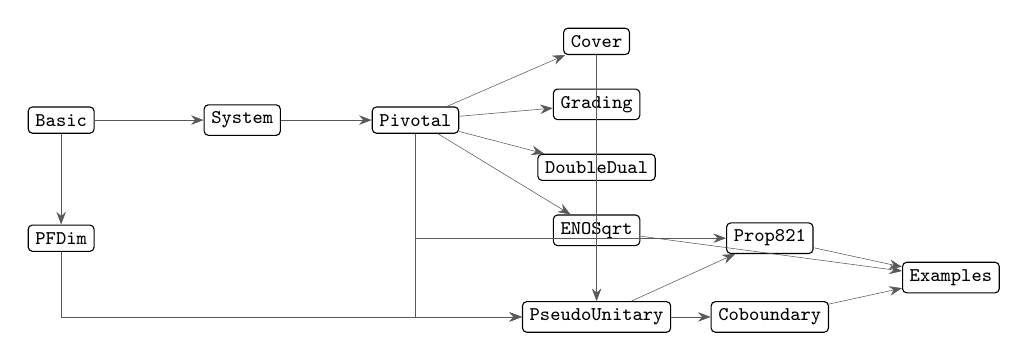
\begin{tikzpicture}[
  >=Stealth,
  box/.style={draw, rounded corners=1.5pt, font=\scriptsize\ttfamily, inner sep=2.6pt},
  ar/.style={-{Stealth[length=1.6mm]}, very thin, gray!70!black}]
% columns
\node[box] (basic) at (0,0) {Basic};
\node[box] (pf)    at (0,-1.5) {PFDim};
\node[box] (sys)   at (2.3,0) {System};
\node[box] (piv)   at (4.5,0) {Pivotal};
\node[box] (cov)   at (6.8,1.0) {Cover};
\node[box] (grad)  at (6.8,0.2) {Grading};
\node[box] (dd)    at (6.8,-0.6) {DoubleDual};
\node[box] (sqrt)  at (6.8,-1.4) {ENOSqrt};
\node[box] (psu)   at (6.8,-2.5) {PseudoUnitary};
\node[box] (cob)   at (9.0,-2.5) {Coboundary};
\node[box] (p821)  at (9.0,-1.5) {Prop821};
\node[box] (ex)    at (11.3,-2.0) {Examples};
\draw[ar] (basic) -- (sys);
\draw[ar] (basic) -- (pf);
\draw[ar] (sys) -- (piv);
\draw[ar] (piv) -- (cov);
\draw[ar] (piv) -- (grad);
\draw[ar] (piv) -- (dd);
\draw[ar] (piv) -- (sqrt);
\draw[ar] (piv) |- (psu);
\draw[ar] (cov) -- (psu);
\draw[ar] (pf) |- (psu);
\draw[ar] (psu) -- (cob);
\draw[ar] (psu) -- (p821);
\draw[ar] (piv) |- (p821);
\draw[ar] (cob) -- (ex);
\draw[ar] (p821) -- (ex);
\draw[ar] (sqrt) -- (ex);
\end{tikzpicture}
\caption{The import spine of the library (transitive imports suppressed; \code{Sanity},
\code{Step4Checks} and the individual \code{Examples/} files are leaves off this spine).
\code{Examples/} is the umbrella over Fibonacci, Ising, Ostrik, $\Vect^{\omega}_{\Z/2}$,
Fibonacci--Ising and the step-4 checks; Yang--Lee and the pseudo-unitary instances are imported
separately by the audit.}
\label{fig:modules}
\end{figure}

{\small
\begin{longtable}{@{}>{\raggedright\arraybackslash}p{0.21\textwidth}>{\raggedright\arraybackslash}p{0.05\textwidth}>{\raggedright\arraybackslash}p{0.05\textwidth}>{\raggedright\arraybackslash}p{0.60\textwidth}@{}}
\toprule
\textbf{Module} & \textbf{Lines} & \textbf{Decls} & \textbf{Content and status} \\
\midrule
\endfirsthead
\toprule
\textbf{Module} & \textbf{Lines} & \textbf{Decls} & \textbf{Content and status} \\
\midrule
\endhead
\bottomrule
\endlastfoot

\code{Basic} & 229 & 26 & fusion ring, fusion/FP matrices, \code{IsPFEigenvector}, \code{FPData},
global dimension. Complete; \code{FPData} is a hypothesis. \\
\code{System} & 451 & 19 & \code{FusionSystem}: $F$, \code{Finv}, snakes, $J$; $\Vect_{\Z/2}$
inhabitant with the 512-tuple pentagon. Complete. \\
\code{Pivotal} & 191 & 21 & \code{PivotalStructure}, \code{dim}, \code{IsSpherical},
\code{isSpherical_iff}, \code{pVal_dual}. Complete. \\
\code{PFDim} & 49 & 5 & \code{PFUnique}, $\varphi$ and its uniqueness. Complete (conditional on
\code{FPData}). \\
\code{Cover} & 128 & 8 & \code{S4Data}, \code{CoverObj}, forgetful functor,
\code{coverGlobalDim_double}. Scaffolding: no \code{PivotalStructure} on the cover yet. \\
\code{Grading} & 153 & 8 & universal grading, \code{pVal_dual}, two \code{def}s recording
open targets. Formerly three axioms; now axiom-free. \\
\code{DoubleDual} & 155 & 9 & the older derived twist in the strict self-dual normalisation.
Lags the $\psi$-derivation; to be rewritten against \code{Finv}. \\
\code{Coboundary} & 331 & 15 & \code{twistNorm}, \code{dim_eq_twistNorm},
\code{eno823_of_twistNorm} and its converse; the pointed \code{KappaMultiplicative} layer
retained for reference. Complete. \\
\code{Prop821} & 474 & 21 & cyclic symmetry, \code{fpdim_char}, the weighted-norm bound, the
equality case, \code{tMatrix}, \code{mult_iff_twist}. Complete modulo \code{DimEigen}. \\
\code{PseudoUnitary} & 452 & 37 & \code{ENO823}, \code{ENO823Exact}, \code{IsPseudoUnitary},
\code{IsPseudoUnitaryPivotal}, \code{eno823_of_pseudoUnitary}, \code{pivotal_ext}. Complete as
a conditional reduction. \\
\code{ENOSqrt} & 232 & 13 & \code{SqrtData}, $b$, \code{Tmat}, $d$, \code{b_sq},
\code{trace_iff}, \code{toPivotal}. Complete; existence of $a$ is assumed. \\
\code{Sanity}, \code{Step4Checks} & 136, 147 & 8 & numerical and consistency checks. Complete;
imported by the umbrella. \\
\code{Examples/FibonacciIsing} & 951 & 115 & Fibonacci and Ising over $\R$: every field proved,
spherical, $\dim = \FPdim$. Complete; $\sim$100\,s. \\
\code{Examples/YangLee} & 419 & 39 & the refutation of the un-hypothesised target. Complete. \\
\code{Examples/VecZ2Twisted} & 86 & 11 & two pivotal structures, $\dim g = \pm 1$. Complete. \\
\code{Examples/Ostrik} & 154 & 21 & the rank-three ring $K(1,0,1)$ and its \code{FPData}. Complete. \\
\code{Examples/}$\cdots$ & 638 & 38 & Fibonacci, Ising, pseudo-unitary instances, $Z/3$ note. \\
\code{MathlibPatches} & 55 & 0 & stubs for \#42150 and the PF chain. Stub: WP0/WP5. \\
\midrule
\textbf{Total} & \textbf{5{,}231} & \textbf{414} & 23 files; build 3{,}032 jobs; audit 73 declarations. \\
\end{longtable}
}

\section{The audit protocol}\label{app:audit}

The protocol is a sequence of gates applied to every declaration before it is merged. Its purpose
is to catch the failure modes F1--F4 of \S\ref{sec:fidelity}, none of which is caught by a
successful build.

\paragraph{Gate 1 --- Inhabitation.} Every structure introduced gets a witness in the same
commit, and the witness is a case from the literature or a standard construction, not a
degenerate one. For \code{FusionSystem} the witness is $\Vect_{\Z/2}$; for
\code{PivotalStructure} the witnesses are $p \equiv 1$ on a datum with $J \equiv 1$ (Fibonacci,
Ising, $\Vect_{\Z/2}$) and a \emph{nonconstant} $p$ on a datum with nontrivial $J$: the pointed
$\Vect^{\omega}_{(\Z/2)^{2}}$ datum with the honest twist $J = \delta(\kappa)$ and
$p_i = 1/\kappa_i$, spherical with $\dim \equiv 1 = \FPdim$. A constant $p$ cannot witness a
nontrivial-$J$ datum --- through \code{p_mon}, $p \equiv 1$ forces $J = 1$ on every active
channel, so the pairing an earlier draft of this gate requested is contradictory --- and until
the $(\Z/2)^{2}$ witness is kernel-checked (WP3 Task~3.4) the nontrivial-$J$ slot of this gate
is unfilled and the pivotal layer counts as unwitnessed. A structure with no witness is not
merged.

\paragraph{Gate 2 --- Sharpness.} Every hypothesis is either used essentially or is recorded as
unused. A hypothesis $H$ is \emph{used essentially} if dropping it makes the statement false on a
witness. The two witnesses carried for this purpose are Yang--Lee (dropping pseudo-unitarity) and
$\Vect^{\omega}_{(\Z/2)^2}$ (dropping multiplicativity). Where no counterexample is known, the
declaration says so.

\paragraph{Gate 3 --- Correspondence.} Each theorem is entered in the statement-to-source table
with (i) the source, (ii) the source's numbering in the edition used, (iii) the quantifiers and
the carrier, (iv) any hypothesis of the source that is absent and why. The ENO numbering trap
(8.23 in the Annals, 8.22 on the arXiv) is recorded there. This is the gate a proof assistant
cannot automate, and the only one that catches drift.

\paragraph{Gate 4 --- Axiom audit, enforcing.} \code{AxiomAudit.lean} prints the axioms of
every exported theorem, but printing is a \emph{report}, not a gate: the earlier instruction
--- run the print and \code{grep} its output --- cannot fail on a Lean error or on an
out-of-budget dependency that prints after one, and a non-zero exit from \code{grep -v} usually
meant \emph{success}. The gate is a checked-in script, \code{tools/audit-gate.sh}, whose
contract is: exit non-zero if (i) \code{lake env lean AxiomAudit.lean} exits non-zero or its
output contains an error (a \texttt{\#print axioms} applied to an \code{axiom} declaration
itself errors, and a name whose module is not imported returns \texttt{Unknown constant}; both
have been mistaken for real findings in this project); (ii) any audited declaration depends on
an axiom outside \texttt{[propext, Classical.choice, Quot.sound]} (strict subsets are within
budget); or (iii) any output line is not a recognised audit line. The script:
\begin{verbatim}
#!/bin/sh
# tools/audit-gate.sh -- Gate 4: enforcing axiom audit.
# Lives at FusionCategory/tools/audit-gate.sh; runnable from anywhere.
set -e
cd "$(dirname "$0")/.."
lake build
out=$(mktemp); trap 'rm -f "$out"' EXIT
lake env lean AxiomAudit.lean > "$out" 2>&1 || { cat "$out"; exit 1; }
grep -q "error" "$out" && { cat "$out"; exit 1; } || true
awk '
  /^$/ { next }
  /does not depend on any axioms/ { next }
  /depends on axioms: \[/ {
    s = $0; sub(/.*depends on axioms: \[/, "", s); sub(/\].*/, "", s)
    n = split(s, a, ", ")
    for (i = 1; i <= n; i++)
      if (a[i] != "propext" && a[i] != "Classical.choice" &&
          a[i] != "Quot.sound") { print "GATE 4: out of budget: " $0; exit 1 }
    next }
  { print "GATE 4: unrecognised audit line: " $0; exit 1 }
' "$out"
echo "gate 4: all audited declarations within budget"
\end{verbatim}
Before the gate is trusted it is \emph{self-tested}: on a scratch branch it is run against an
audit file containing one \code{sorry}-proved theorem and one deliberate \code{axiom}, and it
must fail on both. A gate that has never been observed to fail is a report.

\paragraph{Gate 5 --- Build hygiene.} No \texttt{sorry}, no \texttt{axiom}, no bare
\code{module} header, warnings permitted. The full build must pass from a clean tree (WP0 Task
0.2), not merely incrementally.

\paragraph{Gate 6 --- Regression.} Each defect of Table~1 has a named test that fails if the
defect returns: \code{VecZ2.system} (D1), the 512-tuple pentagon (D2),
\code{VecZ2Twisted.system} (D3), \code{swapped_Finv_comp_ne_one} (D4).

\section{The main statements}\label{app:statements}

For reference, the target statements in mathematical form, with their Lean names.

\paragraph{Pseudo-unitarity.} \code{IsPseudoUnitary S h} is the scalar equation
\[
\sum_{i} \kappa_i\,\kappa_{i^*} \;=\; \sum_i f_i^{2},
\]
with no pivotal structure in it.

\paragraph{The bare target.} \code{ENO823 S h} is
\[
\exists\, P : \mathrm{PivotalStructure}\ S,\quad
P.\mathrm{IsSpherical} \ \wedge\ \forall i,\ \dim_P(i) = f_i .
\]

\paragraph{The exact target.} \code{ENO823Exact S h} states: for every pseudo-unitary $S$ there
is a unique pivotal structure $P$ with
\[
P.\mathrm{IsSpherical}, \qquad \forall i,\ \dim_P i > 0, \qquad \forall i,\ \dim_P i = f_i .
\]
The existence is inside the unique existential; a rendering that lists a spherical structure and
then asserts positivity and uniqueness \emph{conditionally} on $\dim_P = f$ is strictly weaker,
and the earlier draft of this appendix did exactly that. It is withdrawn.
In the $\Cx$ statement (WP1 Task~1.1), the conjunct $\dim_P i > 0$ is read through the
positivity predicate of S2 --- $z$ real with $z > 0$ --- and in both the $\R$ and $\Cx$
statements it follows from $\dim_P i = f_i$ with $f_i > 0$; it is kept because the source states
it (Gate~3), not because it is logically independent. The library's current \code{ENO823Exact}
is stated over $\R$; the $\Cx$ restatement is the same rendering under the scalar contract,
with a real \code{FPData} embedded by $\R \to \Cx$.

\paragraph{The conditional form already proved.} \code{IsPseudoUnitaryPivotal P} is the
conjunction
\[
\bigl(\forall i,\ \dim_P i > 0\bigr) \;\wedge\;
\Bigl(\forall i,k,\ \sum_j N_{ij}^{k}\dim_P j = \dim_P i \cdot \dim_P k\Bigr),
\]
and \code{eno823_of_pseudoUnitary} proves that these two conditions on one pivotal dimension,
together with \code{PFUnique}, give \code{ENO823}.

\paragraph{ENO's input.} \code{SqrtData} carries $a \colon \mathrm{Fin}\,n \to \field^\times$
with $a_i^2 = g_i$ and the monoidality of $a^2$ stated against $J^{2}$; then $b$, \code{Tmat} and
$d$ are
\[
b^{ij}_{c} = J^{ij}_{c}\frac{a_i a_j}{a_c},\qquad
T^{ij}_{c} = N^{ij}_{c} b^{ij}_{c},\qquad
d_i = a_i\,\mathrm{coev}_i\,\mathrm{ev}_{i^*},
\]
and \code{trace_iff} states that $d_i d_j = \sum_c T^{ij}_c d_c$ for all $i,j$ is equivalent to
(M) in the duality normalisation $\kappa'_i = \mathrm{coev}_i\,\mathrm{ev}_{i^*}$.

\paragraph{The derived twist.} The object WP3 must construct is
\[
J^{c}_{ab} \;=\; \frac{\psi_{a,b}|_{c}}{\psi_{b^*,a^*}|_{c^*}},
\qquad
\psi_{a,b} \colon \dual{(a\otimes b)} \to \dual b \otimes \dual a ,
\]
with $\psi$ the unique evaluation-intertwining isomorphism. The closed form in terms of $F$ and
the restricted inverse block $M_b^{-1}$ that \texttt{PLAN.md} displays is \emph{retracted there}
and is not quoted as a target; WP3 Task~3.2 derives the closed form and checks it against
Bartlett's Theorem~4.17.

\paragraph{An ASCII rendering of the headline declaration.} The Unicode binders are spelled out;
this is a rendering for readability, not the source, and it reproduces the existential
conjunction of \code{ENO823Exact} verbatim.
\begin{verbatim}
-- the target, as the library actually defines it
def ENO823Exact (S : FusionSystem n R) (hFP : S.ring.FPData) : Prop :=
  IsPseudoUnitary S hFP ->
    exists! P : PivotalStructure S,
      P.IsSpherical /\
      (forall i, 0 < dim P i) /\
      (forall i, dim P i = hFP.fpdim i)
\end{verbatim}
The conditional form \code{eno823_of_pseudoUnitary} replaces the antecedent by
\code{IsPseudoUnitaryPivotal P} for a \emph{given} $P$ together with \code{PFUnique}; it is
weaker than \code{ENO823Exact} precisely in that it assumes a pivotal structure rather than
producing one.

\section{Changes in this revision}\label{app:changes}

The first draft of this proposal was reviewed, and the review found eight substantive errors and
a list of smaller ones. Each is recorded here with the change made, so that the revision can be
checked against the review rather than against itself.

\begin{center}
\small
\begin{longtable}{@{}>{\raggedright\arraybackslash}p{0.05\textwidth}>{\raggedright\arraybackslash}p{0.40\textwidth}>{\raggedright\arraybackslash}p{0.50\textwidth}@{}}
\toprule
& \textbf{Finding} & \textbf{Change} \\
\midrule
\endfirsthead
\toprule
& \textbf{Finding} & \textbf{Change} \\
\midrule
\endhead
\bottomrule
\endlastfoot
1 & The nontrivial double-dual permutation is based on an error: every simple is isomorphic to
its double dual (ENO Prop.~2.1); pivotality is about the monoidal structure. & The permutation is
removed. Remark~\ref{rem:trap} now separates the objectwise statement from the monoidal one;
WP1 records the label question as closed; failure mode F3 no longer cites it. \\
2 & The promised unconditional theorem exceeds the stated scope (multiplicities, the
quadruple-dual theorem, complex scalars). & \S\ref{sec:scope} states (S1)--(S4); $g$ is a
hypothesis or Bartlett's Theorem~3.28; complex scalars are a WP1 task; the abstract says
``multiplicity-free, characteristic zero''. \\
3 & The analytic package (old WP3, now WP4) misstates the phase correction: $\sigma$ is a tensor
automorphism of the identity, $\tau$ is an ordinary natural automorphism, and $\sigma$ need not be
sign-valued. & WP4 Task~4.5 rewritten with the two steps correctly typed, including the observation that a monoidal character
leaves the defect $b$ unchanged; \S\ref{sec:prelim} and \S\ref{sec:refute} corrected. \\
4 & The square-root criterion for pivotality is invalid, and the cover is an equivariantization.
& WP5 Task~5.3 withdraws the criterion and the no-2-torsion corollary, with the
$\Vect_{\Z/2}$ counterexample; the cover is restated as an equivariantization. \\
5 & The displayed exact target omits existence. & Appendix~\ref{app:statements} reproduces
\code{ENO823Exact} verbatim, including the existential conjunction, and records the weaker
rendering as withdrawn; WP1 Task~1.5 makes this a proof obligation. \\
6 & $X^{2} = \one + 2X$ has no categorification over $\Cx$; a determinant or trace does not make
the general twist scalar. & WP7 Task~7.3 turns the ring into a negative test citing
\cite{OstrikRank2}; \S\ref{sec:tech-mult} states that the condition is an operator equality on
each multiplicity space, with no scalar reduction. \\
7 & The twist package (old WP2, now WP3) reproduces a retracted $\Omega$ formula, and the cyclic
census is vacuous. & WP3 opens
with the retraction, takes the closed form as a task rather than an input, and requires four
genuinely non-trivial cocycles, kernel-checked; the carry-cocycle bug is recorded. \\
8 & The claim about the \emph{number} of pivotal structures is overstated. & The abstract,
Theorem~\ref{thm:vec} and its discussion now claim only that the \emph{dimension function} is not
determined by the ring, and note that the set of structures is a torsor once one exists. \\
\midrule
a & The triangle axiom is derivable, not independent. & WP1 Task~1.2 proves $t = t^{2} \Rightarrow
t = 1$ from the pentagon and invertibility. \\
b & The twist coherence needs the nonzero-entry qualification. & WP1 Task~1.3 states it, citing
Bartlett's Corollary~3.26, and derives the F-free form only on the support. \\
c & (C)$\Rightarrow$(K) is not available in the signature. & Figure~\ref{fig:logic} redrawn: (C)
and (M) are marked necessary and not sufficient, with the pointed false-$J$ datum as the witness;
the missing implication is attributed to the reconstruction and the twist. \\
d & $\FPdim(\C) = \sum_i f_i^{2}$, without the extra square. & Corrected in \S2.2. \\
e & The pseudo-unitarity definition is circular. & Definition~\ref{def:pseudo} now uses ENO's
squared norms, available before pivotality, with the equivalence to (5) as a lemma. \\
f & The cyclic symmetry is missing a dual. & Corrected to $N_{ij}^{k} = N_{j k^*}^{i^*}$, the
\code{cyclic1} statement. \\
g & EGNO attribute the theorem to Proposition~9.5.1. & Corrected in Theorem~\ref{thm:eno823} and
\S\ref{sec:prior}, with EGNO's own note identifying it with ENO~8.23. \\
h & Higher indicators are cyclotomic integers, not integral by sphericity. & Corrected in
\S\ref{sec:prior}. \\
\end{longtable}
\end{center}

\section{Changes in the second revision (v1.2)}\label{app:changes2}

The revised proposal was reviewed a second time, and the review found five substantive defects
and one structural instruction. Each is recorded here with the change made, so that this
revision can be checked against the review rather than against itself.

\begin{center}
\small
\begin{longtable}{@{}>{\raggedright\arraybackslash}p{0.05\textwidth}>{\raggedright\arraybackslash}p{0.40\textwidth}>{\raggedright\arraybackslash}p{0.50\textwidth}@{}}
\toprule
& \textbf{Finding} & \textbf{Change} \\
\midrule
\endfirsthead
\toprule
& \textbf{Finding} & \textbf{Change} \\
\midrule
\endhead
\bottomrule
\endlastfoot

1 & WP1 mishandled zero associator entries: \code{F_support} and \code{J_ne_zero} were said to
guarantee nonzero $F$ on admissible channels. They do not --- \code{F_support} forces zeros off
the channels only, and \code{J_ne_zero} is a statement about $J$. & Task~1.3 rewritten: every
cancellation carries an explicit nonzero side condition $h_F$, or the $F$-factors are retained
in the law; no proof derives nonvanishing from the support axioms. \\

2 & ``A field of characteristic zero'' cannot carry the analytic theorem: it supplies no
absolute values, no square roots, no positivity; and a remaining reference derived positivity
from a Hermitian structure. & The scalar contract (S2, Task~1.1): algebraic layer over a
characteristic-zero field, analytic theorem over $\Cx$ only, with real \code{FPData} embedded,
complex moduli, and positivity defined once; the Hermitian description removed from
\S\ref{sec:whatdone}, WP4, \texttt{PLAN.md} and the Lean doc comments. \\

3 & WP2 Task~2.3 asked reconstruction to identify the carried field $S.J$ with the double-dual
tensorator --- an identification the false-$J$ datum refutes. & Task~2.3 rewritten:
reconstruction defines \code{derivedJ} independently; the relation to a carried $J$ is the
explicit hypothesis \code{J_match}, discharged per instance (Task~3.3), or the field is
replaced by the derived definition. \\

4 & Gate 1 requested $p \equiv 1$ on a nontrivial-$J$ datum --- contradictory, since
\code{p_mon} then forces $J = 1$ on every active channel; and Gate 4's \code{\#print axioms}
plus \code{grep} is a report that cannot fail on a Lean error or an out-of-budget dependency. &
Gate 1 names a nonconstant witness ($p_i = 1/\kappa_i$ on the $(\Z/2)^{2}$ datum with
$J = \delta(\kappa)$) and records the slot as unfilled until kernel-checked; Gate 4 is the
enforcing script \code{tools/audit-gate.sh} with three failure conditions and a negative
self-test. \\

5 & Three contradictory instructions: \texttt{PLAN.md} still requested a nontrivial double-dual
label permutation; Task~1.5 asked for an equivalence with a form it had just withdrawn as
strictly weaker; Task~4.5 called the dimension ratios positive where only their squares are
determined. & The request is withdrawn (ENO Prop.~2.1; \texttt{PLAN.md} now records the
closure); Task~1.5 names its forms --- exact $\leftrightarrow$ bare via \code{pivotal_ext} and
FPdim positivity, the withdrawn rendering is not a target; Task~4.5 states the squared identity
and defers the signs to the $\tau$-step. \\

6 & Structure: the review asked for a first delegation batch and an explicit source of truth
before any unattended run. & \S\ref{sec:batch}: batch B1--B4 (reproduce the clean build,
enforcing axiom audit, repair the cocycle census, settle the corrected signature and theorem
statement), the source-of-truth paragraph superseding \texttt{PLAN.md}, and the holding rule
that gates WP2--WP4 on the batch's review. \\

\end{longtable}
\end{center}

\end{document}
